\documentclass[]{article}

\def\nno{\nonumber}
\def\bfE{\mbox{\boldmath$E$}}
\def\bfG{\mbox{\boldmath$G$}}
\def \p{\partial}
\usepackage{epsfig, color}
\usepackage{color,graphicx}
\usepackage{amsfonts}
\usepackage{color}
\usepackage{amsmath}
\usepackage{amssymb}
\usepackage{amsthm}
\usepackage{natbib}
\usepackage{fancybox}
\usepackage{ulem}
\usepackage{subfigure}
\usepackage{multirow}
\usepackage{bbm}
\usepackage{enumerate}
\usepackage{rotating}
\usepackage{float}
\usepackage{epstopdf}
\usepackage{tcolorbox}
\usepackage{mdframed}
\usepackage{framed}
\usepackage{graphbox}
\usepackage{makecell}
\usepackage{diagbox}
\usepackage{booktabs}

%\usepackage{refcheck}

\allowdisplaybreaks[4]

\newtheorem{definition}{\hspace{6mm}Definition}[section]
\newtheorem{theorem}{\hspace{6mm}Theorem}[section]
%\newtheorem{lemma}{\hspace{6mm}Lemma}[section]
\newtheorem{remark}{\hspace{6mm}Remark}[section]
\newtheorem{lemma}[theorem]{\hspace{6mm}Lemma}
%\newtheorem{remark}[theorem]{Remark}
\newtheorem{example}{\textsc{Example}}[section]
\newtheorem{proposition}{\hspace{6mm}Proposition}[section]
\newtheorem{algorithm}{Algorithm}
\renewcommand{\(}{\left(}
\renewcommand{\)}{\right)}
\newcommand{\bm}[1]{\mbox{\boldmath{$#1$}}}
\def\cred{\color{red}}
\def\cblue{\color{blue}}
\def\cgreen{\color{green}}

%opening
\title{Deep signature transforms for rough volatility model}
\author{}
\date{}

\begin{document}

\maketitle

%\begin{abstract}
%
%\end{abstract}

\section{Preliminary numerical experiments}
\subsection{Implementation details}\label{sec1}
We follow \cite{Lyons_2019_DeepSignature} to design these experiments. Details for each models we used as follows and all models used a sigmoid as a final nonlinearity, so as to map in to $(0, 1)$:
\begin{itemize}
	\item The Feedforward model was a simple fully connected neural network with $3$ hidden layers of $16$ neurons each.
	\item The Neural-Sig model shown in Figure~\ref{fig-structure-neuralsig} – which is essentially the same model as the Feedforward model, except that the data has the signature applied as feature transformation first – featured hidden layers of sizes $64,\, 64,\, 32,\, 32,\, 16,\, 16$ respectively. 
	\begin{figure}[H]
		\centering
		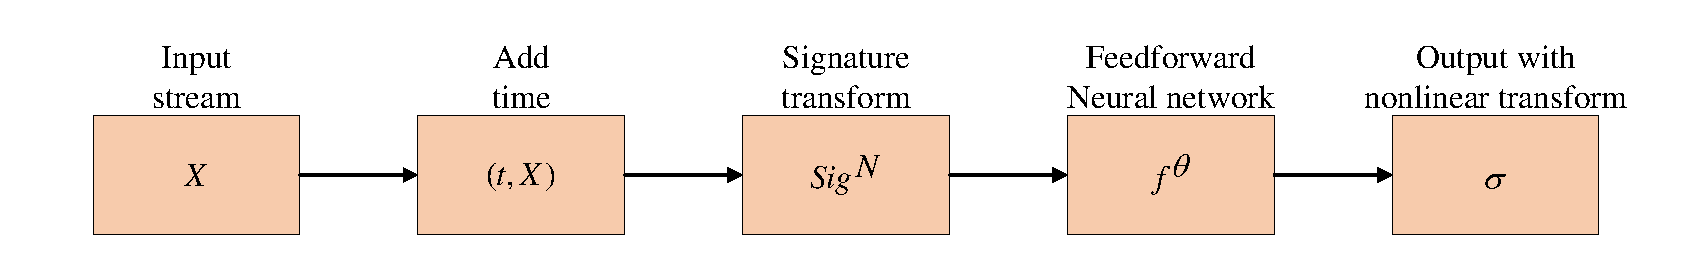
\includegraphics[width=0.9\textwidth]{fig//structure//Neural-Sig.pdf}
		\caption{Structure of neural signature model. Trainable parameters: $\theta$. }
		\label{fig-structure-neuralsig}
	\end{figure}
	\item The RNN model shown in Figure~\ref{fig-structure-rnn} is two recurrent neural networks, the first comprised of dense layers of sizes $64,\, 64,\, 32$ and output size $6$, and the second comprised of dense layers of size $32,\, 32,\, 32$, and output size $5$. The first network sweeps across the input data relatively slowly, with a stride of $2$, whilst the second network sweeps across the result of the first network more quickly, with a stride of $4$. In this way it may capture information from the input data at multiple timescales; part of the challenge of fractional Brownian motion is the existence of long-range dependencies.
	\begin{figure}[H]
		\centering
		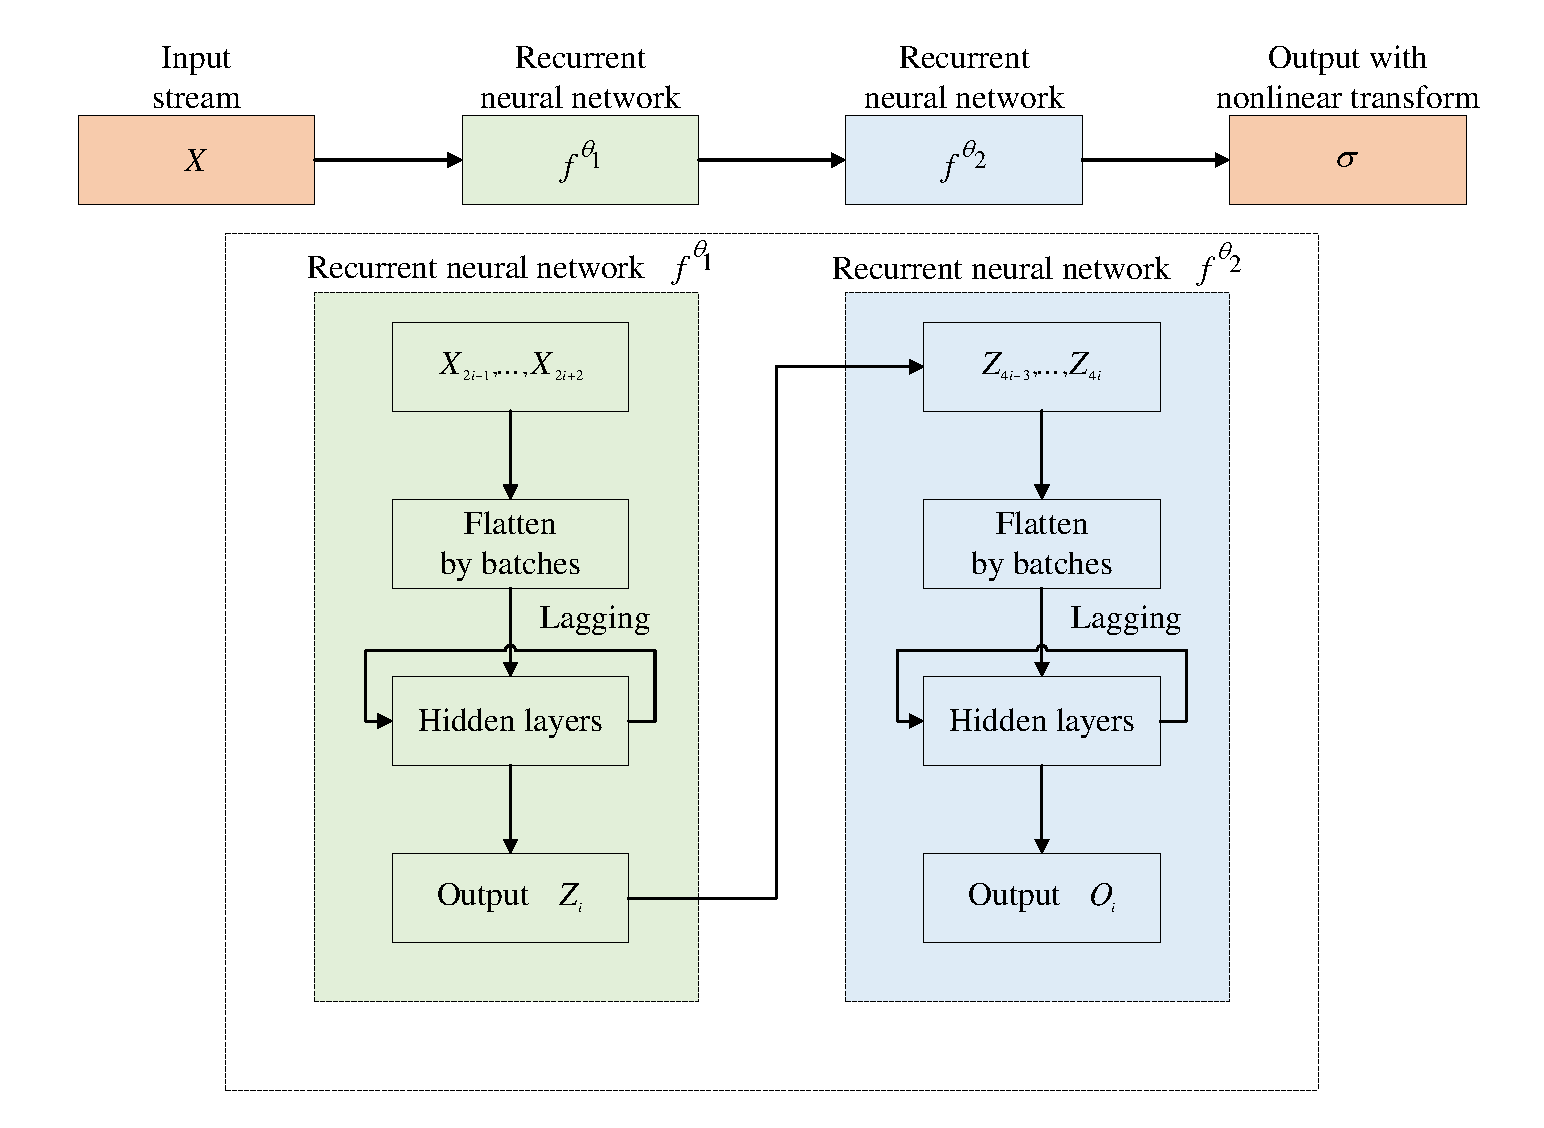
\includegraphics[width=0.9\textwidth]{fig//structure//RNN.pdf}
		\caption{Structure of RNN model. Trainable parameters: $\theta_1$ and $\theta_2$. }
		\label{fig-structure-rnn}
	\end{figure}
	\item The LSTM and GRU models both featured two recurrent layers each of size $32$, and swept across the raw data with a stride of $1$.
	\item DeepSigNet model shown in Figure~\ref{fig-structure-deepsignet} featured a single Neural-Lift-Signature block, where the neural component was given by a single convolutional layer with $3$ channels and kernel size $3$, the lift was the trivial lift, and the signature was truncated as $N = 3$. The neural component also preserved the original time-augmented stream of data, so that in some sense the neural component has $3$ extra channels corresponding to time and value. On top of this a feedforward neural network with $5$ hidden layers of size $32$ was placed. Thus this model is very similar to the Neural-Sig model, except that a small learnable transformation was allowed before the signature. The difference in their performance highlights the value of learning a transformation before using the signature. (Without which the Neural-Sig model is merely outperformed by some non-signature based models.)
	\begin{figure}[H]
	\centering
	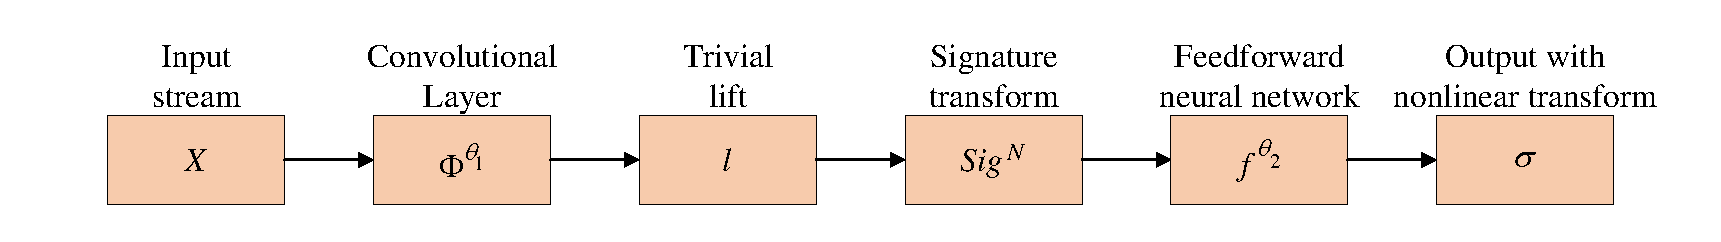
\includegraphics[width=0.9\textwidth]{fig//structure//DeepSigNet.pdf}
	\caption{Structure of DeepSigNet model. Trainable parameters: $\theta_1$ and $\theta_2$. }
	\label{fig-structure-deepsignet}
\end{figure}
	\item DeeperSigNet featured three Neural-Lift-Signature blocks. The neural component of the first block was a small feedforward network with $2$ hidden layers of size 16 and an output layer of size $3$, swept across the length of the stream; its kernel size (how many time-value pairs of the stream it saw at once) was $4$. The original time-augmented stream of data was also preserved by the neural component. The neural components of the other two blocks were recurrent neural networks, featuring $2$ hidden layers of 16 neurons each. The lifts were in every case expanding windows as $l(X)=(X_2,\ldots,X_n)=((x_1,x_2),(x_1,x_2,x_3),\ldots,(x_1,x_2,\ldots,x_n))$ where $X=(x_1,\ldots,x_n)\in\mathcal{S}(\mathbb{R}^d)$. On top of this another recurrent neural network was placed, and the value of its final hidden state used as the output. This final network used $2$ hidden layers of $16$ neurons each.
\end{itemize}

The training set featured $600$ samples whilst the test set featured $100$ samples, each of an instance of fractional Brownian motion sampled at $300$ time steps of $[0, 1]$ and generated by Davies-Harte method. These were split up into batches of $128$ samples, so the last batch is slightly smaller than the others, and every model trained for $100$ epochs.

\subsection{Supervised learning with fractional Brownian motion}
\subsubsection{Reproducing the experiment of the original paper}\label{original exp}
In this example, we reproduce the second experiment of \cite{Lyons_2019_DeepSignature} to train a variety of models to estimate Hurst parameter $H$ from paths of fractional Brownian motion $B^H$. That is, to learn the map $$((t_0, B^H_{t_0}),\ldots,(t_n, B^H_{t_n})) \mapsto H.$$

Here we set $H \in [0.2, 0.8]$ for data sets and every model trained for $100$ epochs. The results are shown in Table~\ref{tab-reproduce} and Figure~\ref{fig-reproduce}. It seems that we did not successfully reproduce the performance gap between the DeepSigNet model and DeeperSigNet model. In addition, the variance of the MSE we obtained is also significantly smaller than the results in the original paper.

\begin{table}[H]
	\caption{Final test mean squared error (MSE) for different models, averaged over 3 training runs, ordered from largest to smallest.}
	\label{tab-reproduce}
	\smallskip
	\centering
	\renewcommand\arraystretch{1.5}
	\resizebox{0.9\textwidth}{!}{\begin{tabular}{l c c c c}
		\toprule
		&\multicolumn{2}{c}{Test MSE} & & \\
		\cline{2-3}
		& Mean & Variance & $\#$Params & CPU time \\
		\cline{2-5}
		LSTM &$3.76 \times 10^{-2}$&$1.40 \times 10^{-5}$&12961&372.00s\\
		Feedforward &$3.21 \times 10^{-2}$&$1.18 \times 10^{-5}$&10209&2.05s\\
		Neural-Sig &$1.37 \times 10^{-2}$&$2.49 \times 10^{-7}$&10097&2.48s\\
		RNN &$6.40 \times 10^{-3}$&$1.11 \times 10^{-5}$&10091&119.86s\\
		GRU &$1.32 \times 10^{-3}$&$1.73 \times 10^{-7}$&9729&291.72s\\
		DeepSigNet &$3.25 \times 10^{-4}$&$5.25 \times 10^{-8}$&9261&48.47s\\
		DeeperSigNet &$3.21 \times 10^{-4}$&$3.52 \times 10^{-8}$&9686&1500.92s\\				
		\bottomrule
	\end{tabular}}
\end{table}

\begin{figure}[H]
	\centering
	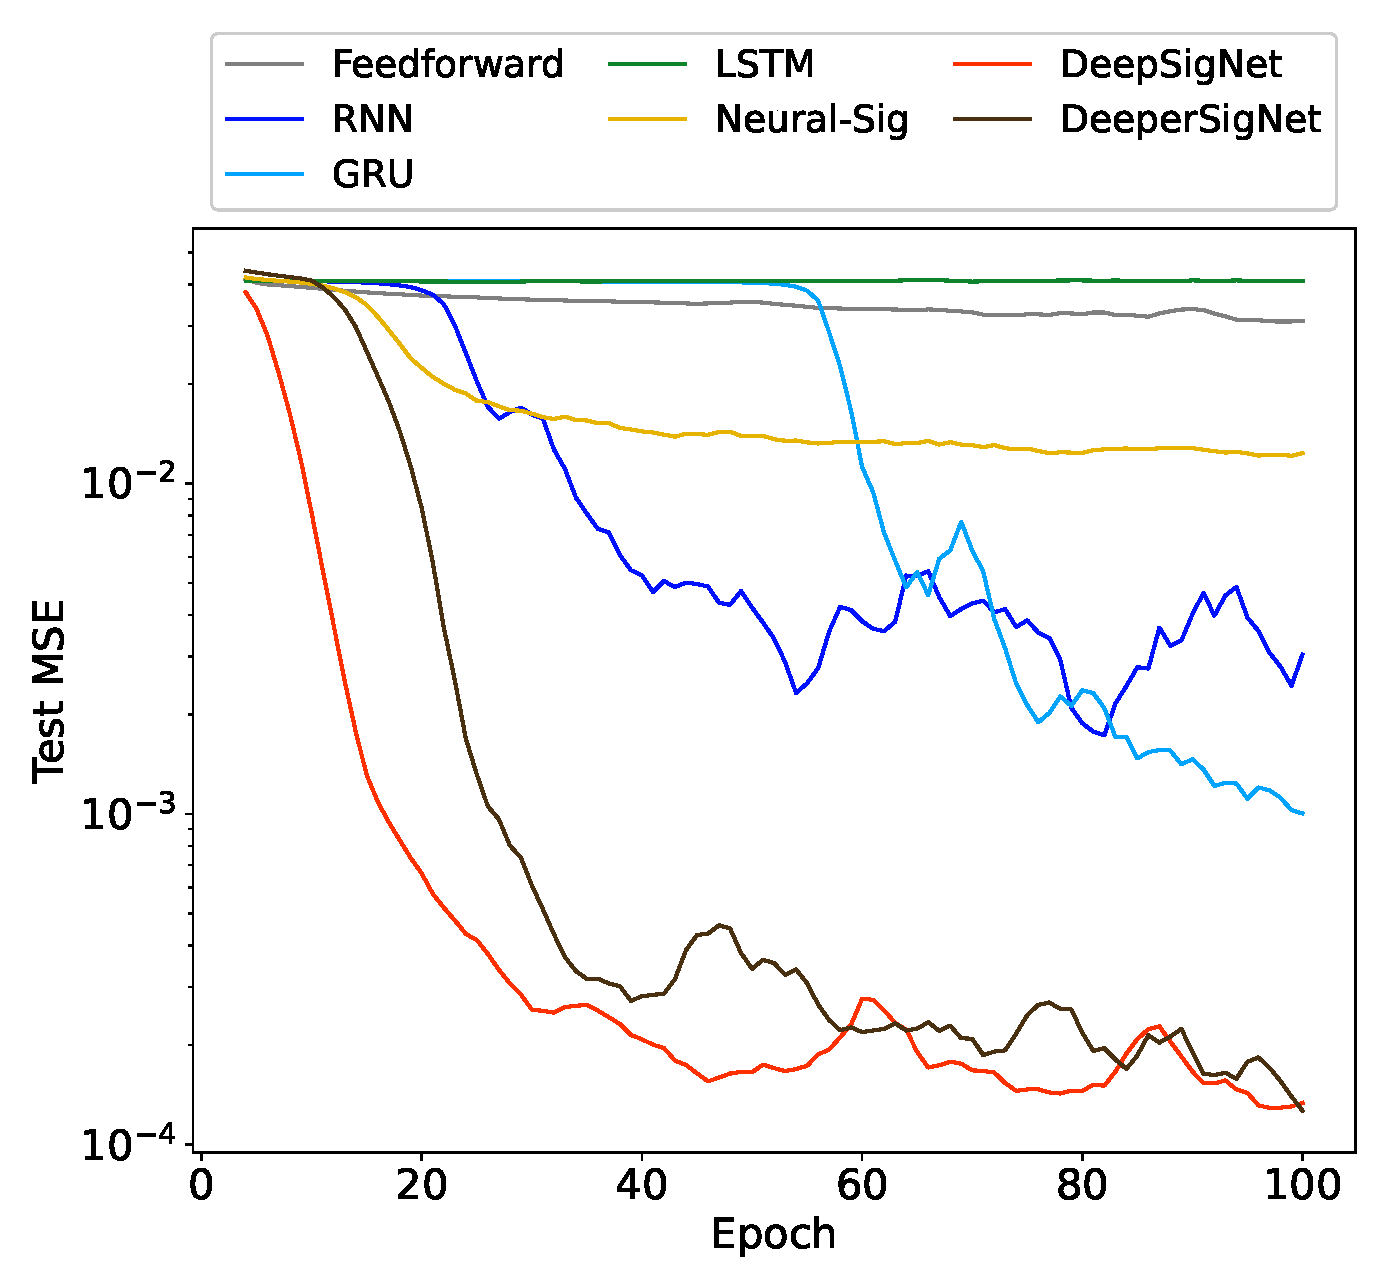
\includegraphics[width=0.32\textwidth]{fig//reproduce//round1.eps}
	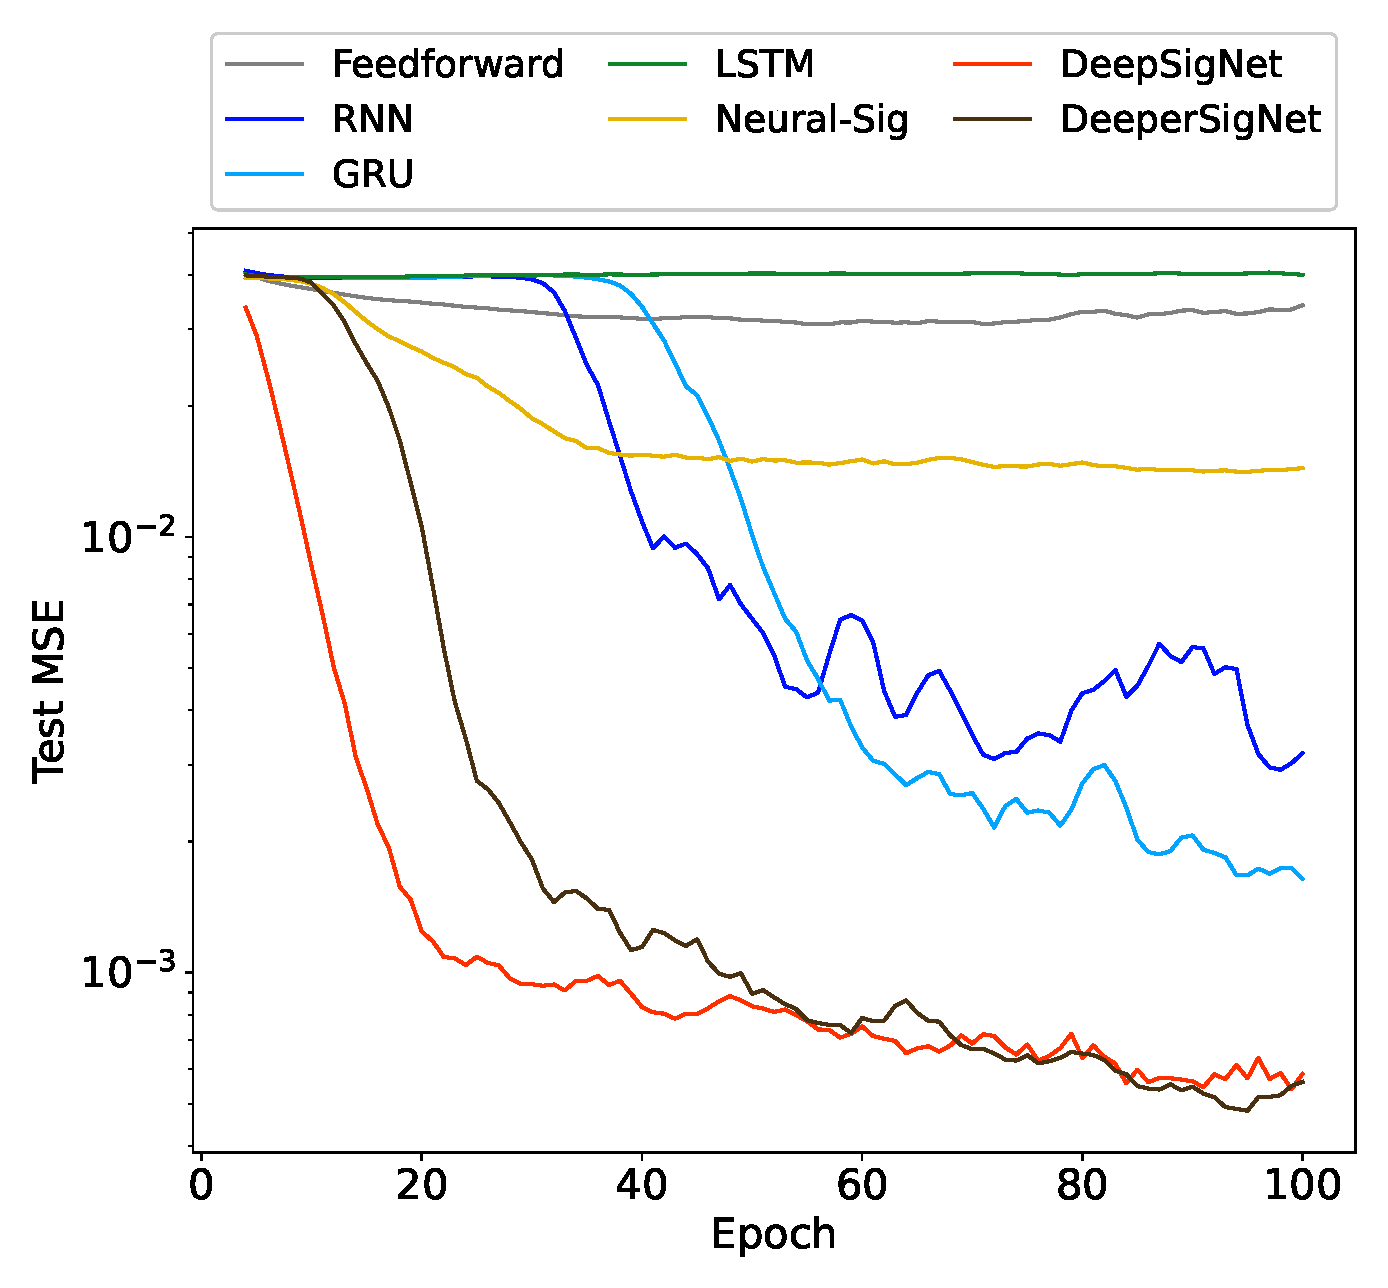
\includegraphics[width=0.32\textwidth]{fig//reproduce//round2.eps}
	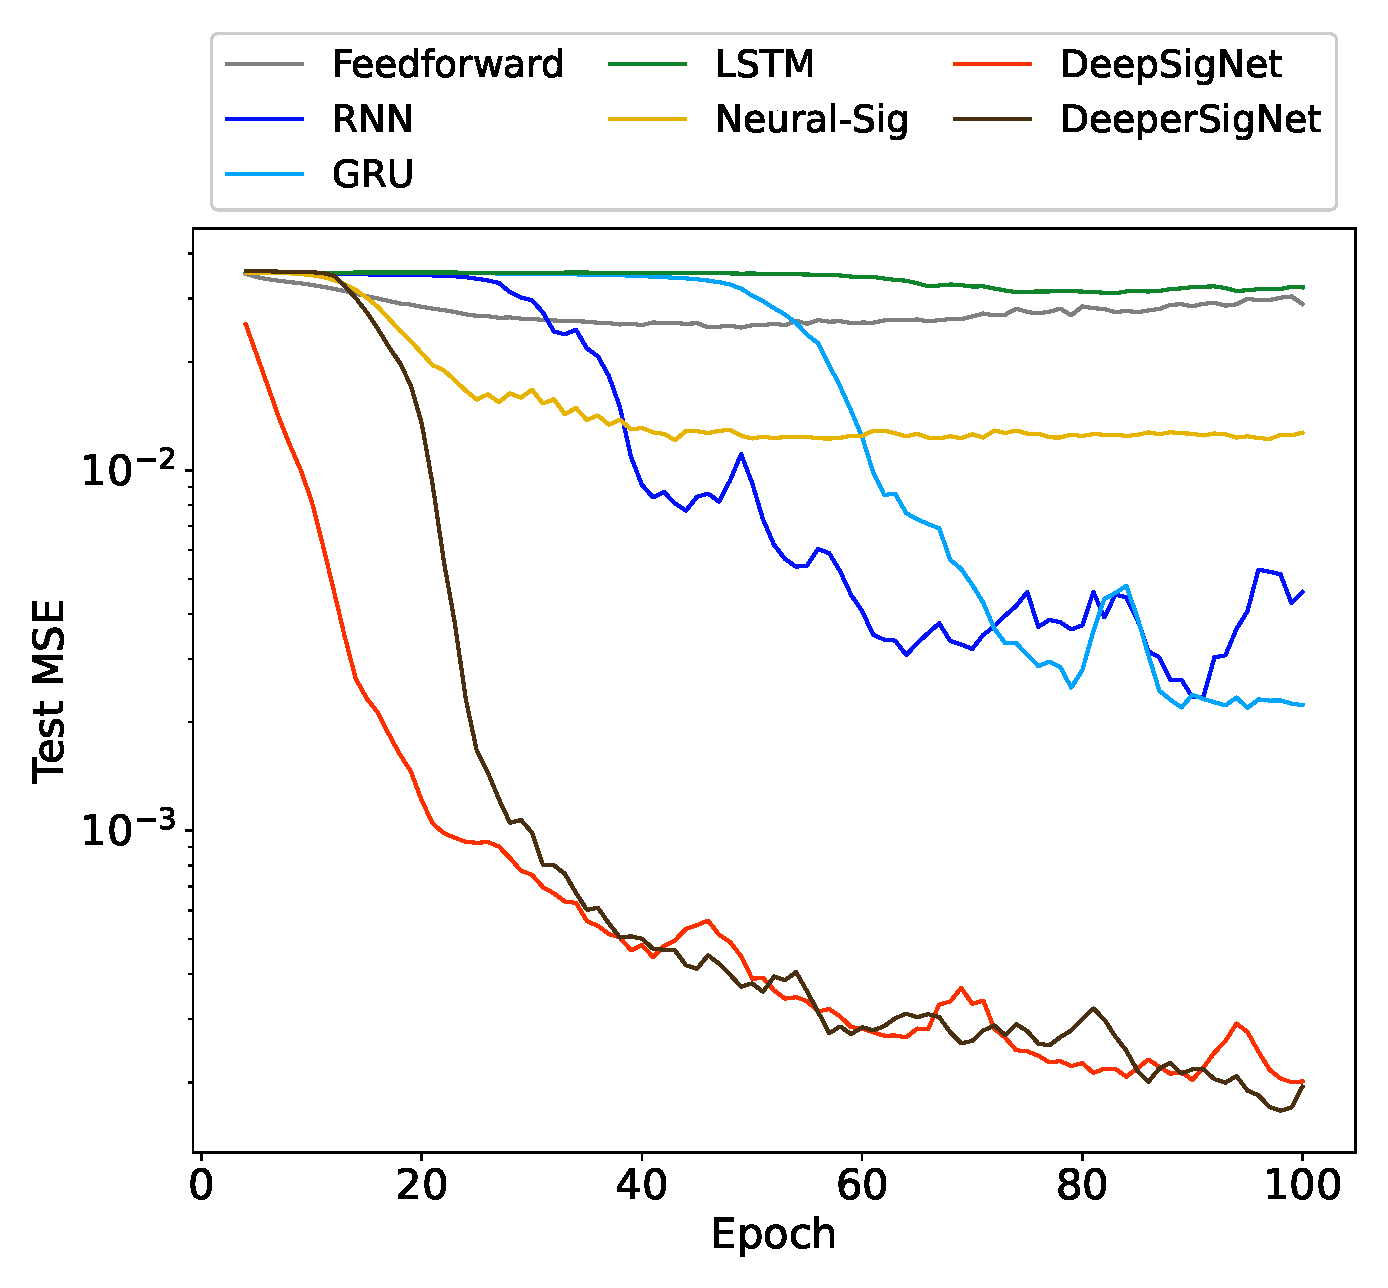
\includegraphics[width=0.32\textwidth]{fig//reproduce//round3.eps}
	\caption{Performance at estimating the Hurst parameter for various models, with and without signatures, for three training runs.}
	\label{fig-reproduce}
\end{figure}


\subsubsection{Adjusting Hurst Parameter Range}
In this example, we slightly modify the previous experiment by adjusting the range of the Hurst parameter value, while keeping all other settings the same. The results are shown in Table~\ref{tab-reproduce-diffH} and Figure~\ref{fig-reproduce-diffH}. The results shows that the DeepSigNet model and DeeperSigNet model performs better for $H\in[0.3, 0.5]$, suggesting that paths are smoother compared to those with $H\in\left(0, 0.2\right]$.

\begin{table}[H]
	\caption{Final test mean squared error (MSE) for different models, averaged over 3 training runs.}
	\label{tab-reproduce-diffH}
	\smallskip
	\centering
	\renewcommand\arraystretch{1.5}
	\resizebox{0.9\textwidth}{!}{\begin{tabular}{l c c c c c}
			\toprule
			& & \multicolumn{2}{c}{Test MSE} & & \\
			\cline{3-4}
			& Hurst parameter & Mean & Variance & CPU time & $\#$Params\\
			\hline
			\multirow{3}{*}{Feedforward} &$\left(0, 0.2\right]$&$5.87 \times 10^{-3}$&$5.77 \times 10^{-7}$&1.92s&\multirow{3}{*}{10209}\\
			&$\left[0.3, 0.5\right]$&$4.85 \times 10^{-3}$&$1.45 \times 10^{-7}$&1.91s&\\
			&$\left(0.5, 0.7\right]$&$3.78 \times 10^{-3}$&$2.17 \times 10^{-7}$&1.89s&\\
			\hline
			\multirow{3}{*}{RNN} &$\left(0, 0.2\right]$&$6.03 \times 10^{-3}$&$5.81 \times 10^{-5}$&118.49s&\multirow{3}{*}{10091}\\
			&$\left[0.3, 0.5\right]$&$1.02 \times 10^{-3}$&$5.73 \times 10^{-8}$&143.84s&\\
			&$\left(0.5, 0.7\right]$&$3.87 \times 10^{-3}$&$5.42 \times 10^{-8}$&143.12s&\\
			\hline
			\multirow{3}{*}{DeepSigNet} &$\left(0, 0.2\right]$&$1.17 \times 10^{-4}$&$3.53 \times 10^{-10}$&47.78s&\multirow{3}{*}{9261}\\
			&$\left[0.3, 0.5\right]$&$8.71 \times 10^{-5}$&$2.24 \times 10^{-10}$&47.91s&\\
			&$\left(0.5, 0.7\right]$&$2.20 \times 10^{-4}$&$7.63 \times 10^{-10}$&56.74s&\\
			\hline
			\multirow{3}{*}{DeeperSigNet} &$\left(0, 0.2\right]$&$1.01 \times 10^{-4}$&$9.15 \times 10^{-11}$&1537.36s&\multirow{3}{*}{9686}\\
			&$\left[0.3, 0.5\right]$&$9.69\times 10^{-5}$&$4.12 \times 10^{-11}$&1499.44s&\\
			&$\left(0.5, 0.7\right]$&$2.74 \times 10^{-4}$&$3.81 \times 10^{-9}$&1508.72s&\\
			\hline
			\multirow{3}{*}{LSTM} &$\left(0, 0.2\right]$&$3.82 \times 10^{-3}$&$2.37 \times 10^{-7}$&205.67s&\multirow{3}{*}{12961}\\
			&$\left[0.3, 0.5\right]$&$4.53 \times 10^{-3}$&$1.54 \times 10^{-7}$&454.39s&\\
			&$\left(0.5, 0.7\right]$&$3.79 \times 10^{-3}$&$3.54 \times 10^{-8}$&410.67s&\\
			\hline
			\multirow{3}{*}{GRU} &$\left(0, 0.2\right]$&$2.21 \times 10^{-4}$&$1.79 \times 10^{-10}$&251.83s&\multirow{3}{*}{9729}\\
			&$\left[0.3, 0.5\right]$&$3.87 \times 10^{-3}$&$9.08 \times 10^{-7}$&326.70s&\\
			&$\left(0.5, 0.7\right]$&$3.83 \times 10^{-3}$&$3.55 \times 10^{-8}$&291.88s&\\
			\hline
			\multirow{3}{*}{Neural-Sig} &$\left(0, 0.2\right]$&$3.13 \times 10^{-3}$&$7.45 \times 10^{-8}$&2.27s&\multirow{3}{*}{10097}\\
			&$\left[0.3, 0.5\right]$&$4.58 \times 10^{-3}$&$4.36 \times 10^{-7}$&2.25s&\\
			&$\left(0.5, 0.7\right]$&$3.23 \times 10^{-3}$&$2.78 \times 10^{-8}$&2.24s&\\
			\bottomrule
	\end{tabular}}
\end{table}

\begin{figure}[H]
	\centering
	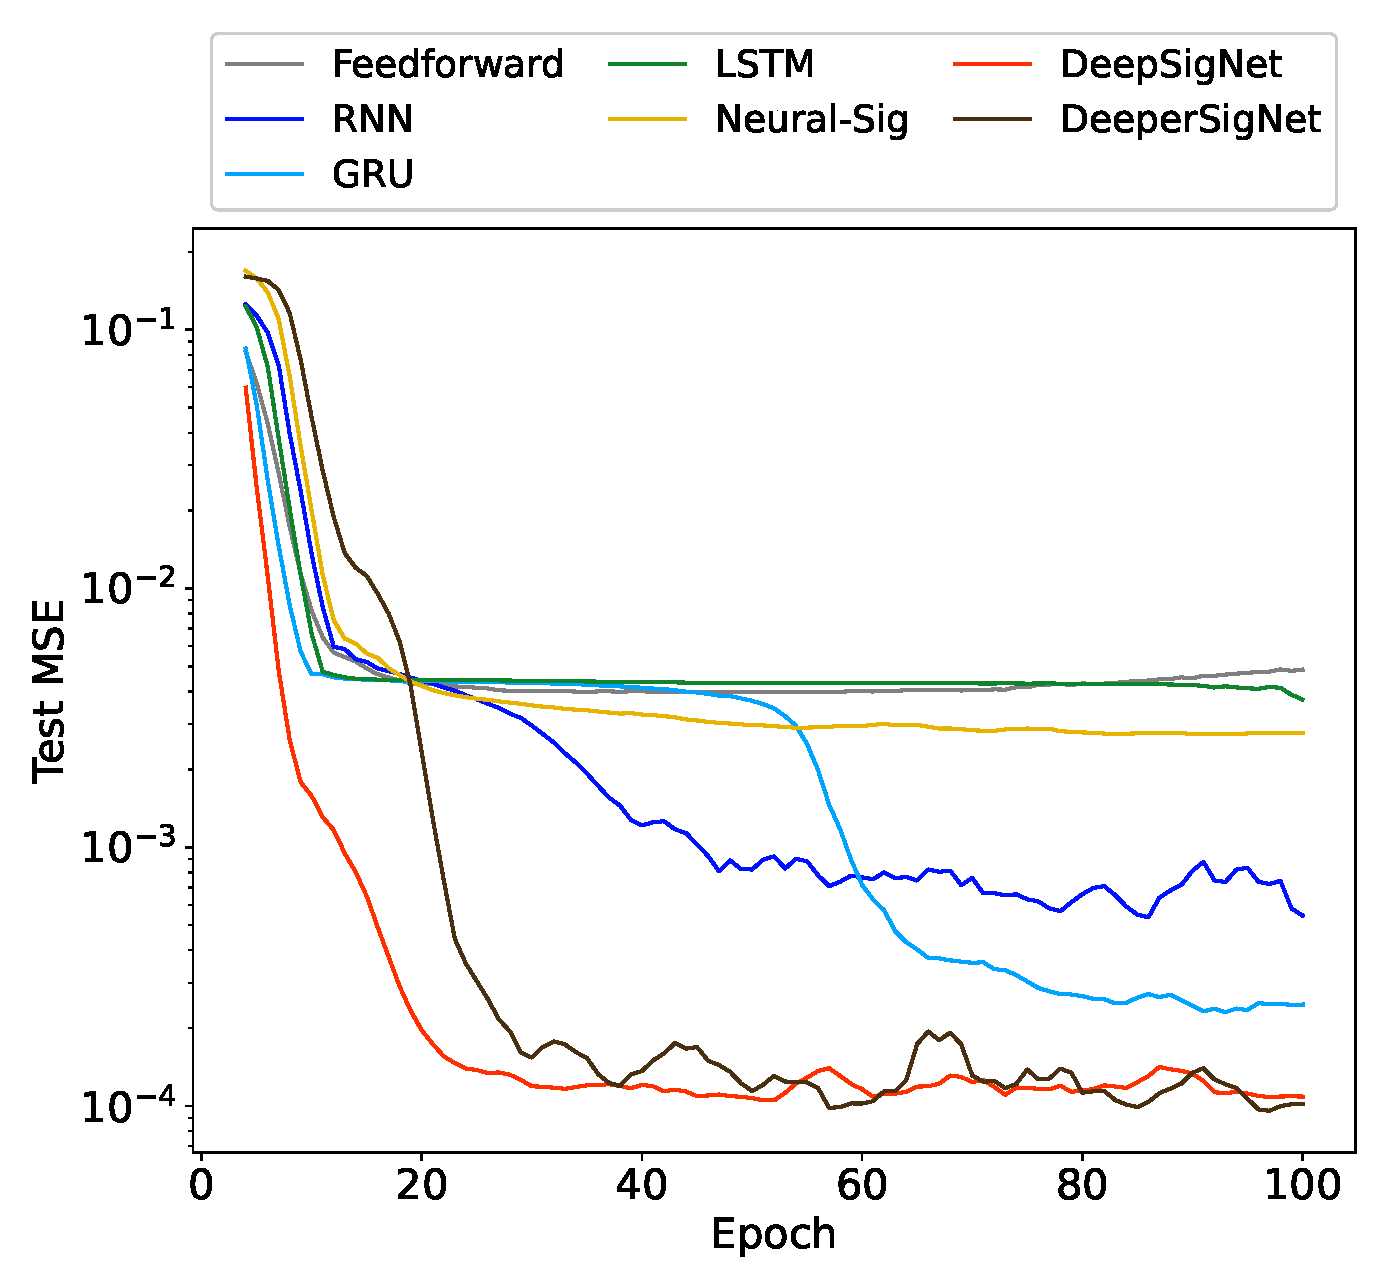
\includegraphics[width=0.32\textwidth]{fig//reproduce//diffH1.eps}
	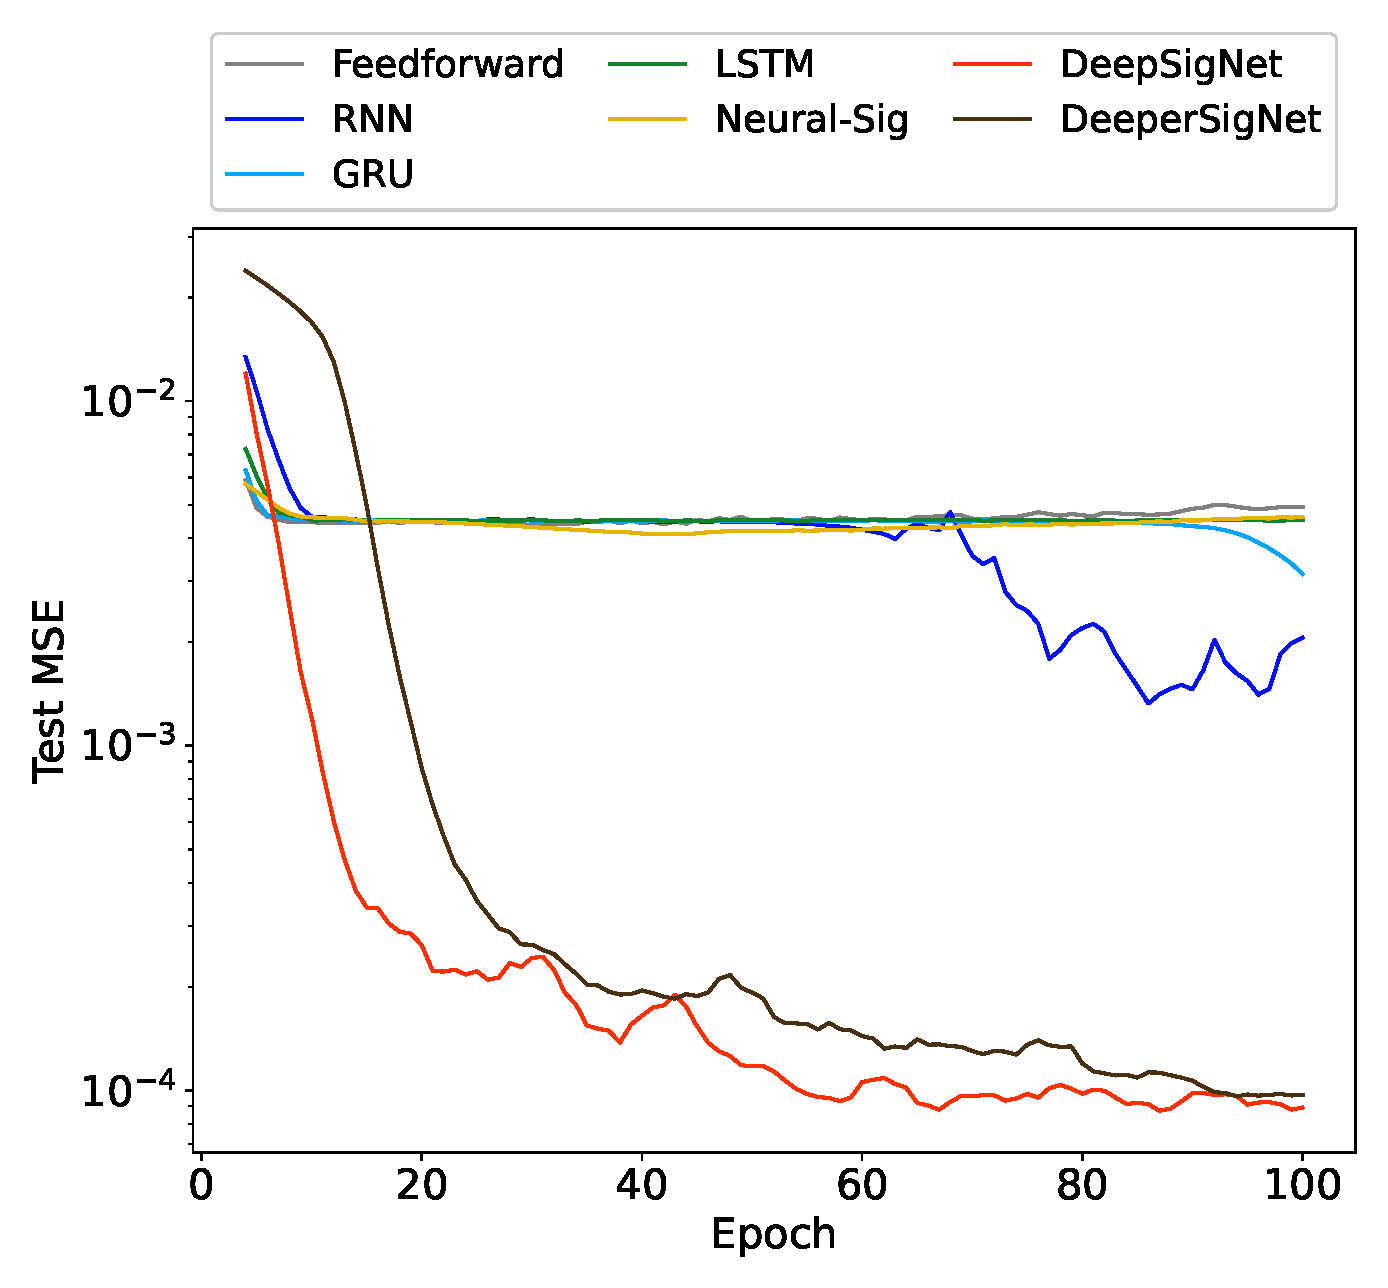
\includegraphics[width=0.32\textwidth]{fig//reproduce//diffH2.eps}
	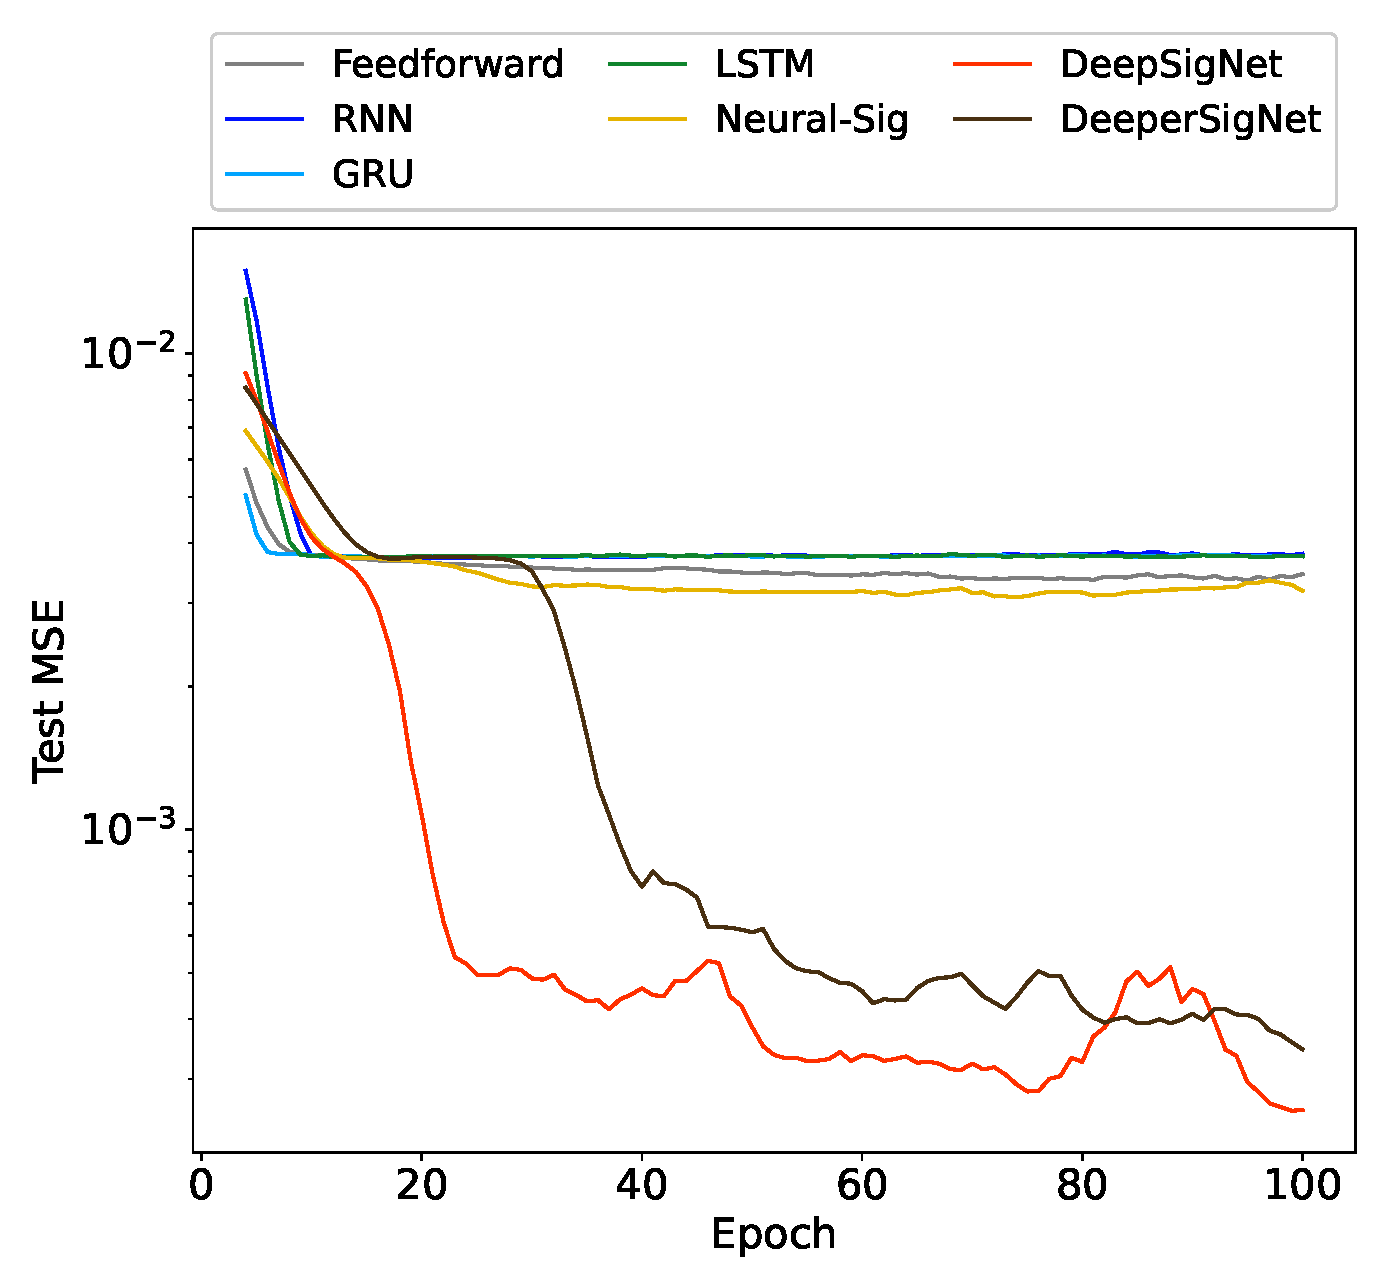
\includegraphics[width=0.32\textwidth]{fig//reproduce//diffH3.eps}
	\caption{Performance at estimating the Hurst parameter for various models, with and without signatures, for a particular (typical) training run. Here, $H\in\left(0, 0.2\right]$ (left); $H\in\left[0.3, 0.5\right]$ (middle); $H\in\left(0.5, 0.7\right]$ (right). }
	\label{fig-reproduce-diffH}
\end{figure}

\subsubsection{Adjusting signature truncation order}
In this example, we try to adjust the signature truncation order for DeepSigNet model, DeeperSigNet model and Neural-Sig model. The results are shown in Table~\ref{tab-reproduce-difforder} and Figure~\ref{fig-reproduce-difforder}. In the case of the Neural-Sig model, the test MSE decreases with the signature truncation order increases. However, for the DeepSigNet model and the DeeperSigNet model, selecting a signature truncation order of $N=3$ or $N=4$ is sufficient.
\begin{table}[H]
	\caption{Final test mean squared error (MSE) for different models, averaged over 3 training runs. In this table, 'null' indicates that the corresponding experiment was not conducted. }
	\label{tab-reproduce-difforder}
	\smallskip
	\centering
	\renewcommand\arraystretch{1.5}
	\resizebox{0.9\textwidth}{!}{\begin{tabular}{l c c c c c}
			\toprule
			&\multicolumn{2}{c}{Test MSE} & & &\\
			\cline{2-3}
			& Mean & Variance & CPU time & $\#$Params &Truncation order\\
			\hline
			DeepSigNet &$2.90 \times 10^{-3}$&$1.14 \times 10^{-8}$&10.11s&4461&\multirow{3}{*}{1}\\
			DeeperSigNet &$1.14 \times 10^{-3}$&$2.79 \times 10^{-8}$&324.07s&2486&\\
			Neural-Sig &$4.09 \times 10^{-3}$&$6.84 \times 10^{-8}$&2.23s&8305&\\
			\hline
			DeepSigNet &$1.15 \times 10^{-4}$&$2.26 \times 10^{-10}$&17.72s&5261&\multirow{3}{*}{2}\\
			DeeperSigNet &$1.23 \times 10^{-4}$&$2.18 \times 10^{-9}$&546.85s&3686&\\
			Neural-Sig &$4.22 \times 10^{-3}$&$1.31 \times 10^{-8}$&2.15s&8561&\\
			\hline
			DeepSigNet &$1.32 \times 10^{-4}$&$1.39 \times 10^{-10}$&48.20s&9261&\multirow{3}{*}{3}\\
			DeeperSigNet &$1.49 \times 10^{-4}$&$1.06 \times 10^{-9}$&1495.74s&9686&\\
			Neural-Sig &$3.04 \times 10^{-3}$&$4.65 \times 10^{-7}$&2.16s&9073&\\
			\hline
			DeepSigNet &$8.51 \times 10^{-5}$&$8.74 \times 10^{-11}$&237.15s&29261&\multirow{3}{*}{4}\\
			DeeperSigNet &$1.11 \times 10^{-4}$&$1.03 \times 10^{-9}$&7361.82s&39686&\\
			Neural-Sig &$2.76 \times 10^{-3}$&$1.57 \times 10^{-7}$&2.35s&10097&\\
			\hline
			DeepSigNet &$1.69 \times 10^{-4}$&$2.94 \times 10^{-9}$&1388.30&129261&\multirow{3}{*}{5}\\
			DeeperSigNet &null&null&null&null&\\
			Neural-Sig &$1.83 \times 10^{-3}$&$3.39 \times 10^{-8}$&2.28&12145&\\
			\hline
			DeepSigNet &$2.76 \times 10^{-4}$&$8.75 \times 10^{-9}$&8629.09s&629261&\multirow{3}{*}{6}\\
			DeeperSigNet &null&null&null&null&\\
			Neural-Sig &$1.55 \times 10^{-3}$&$6.07 \times 10^{-9}$&4.28s&16241&\\
			\bottomrule
	\end{tabular}}
\end{table}


\begin{figure}[H]
	\centering
	\subfigure[$N=1$.]{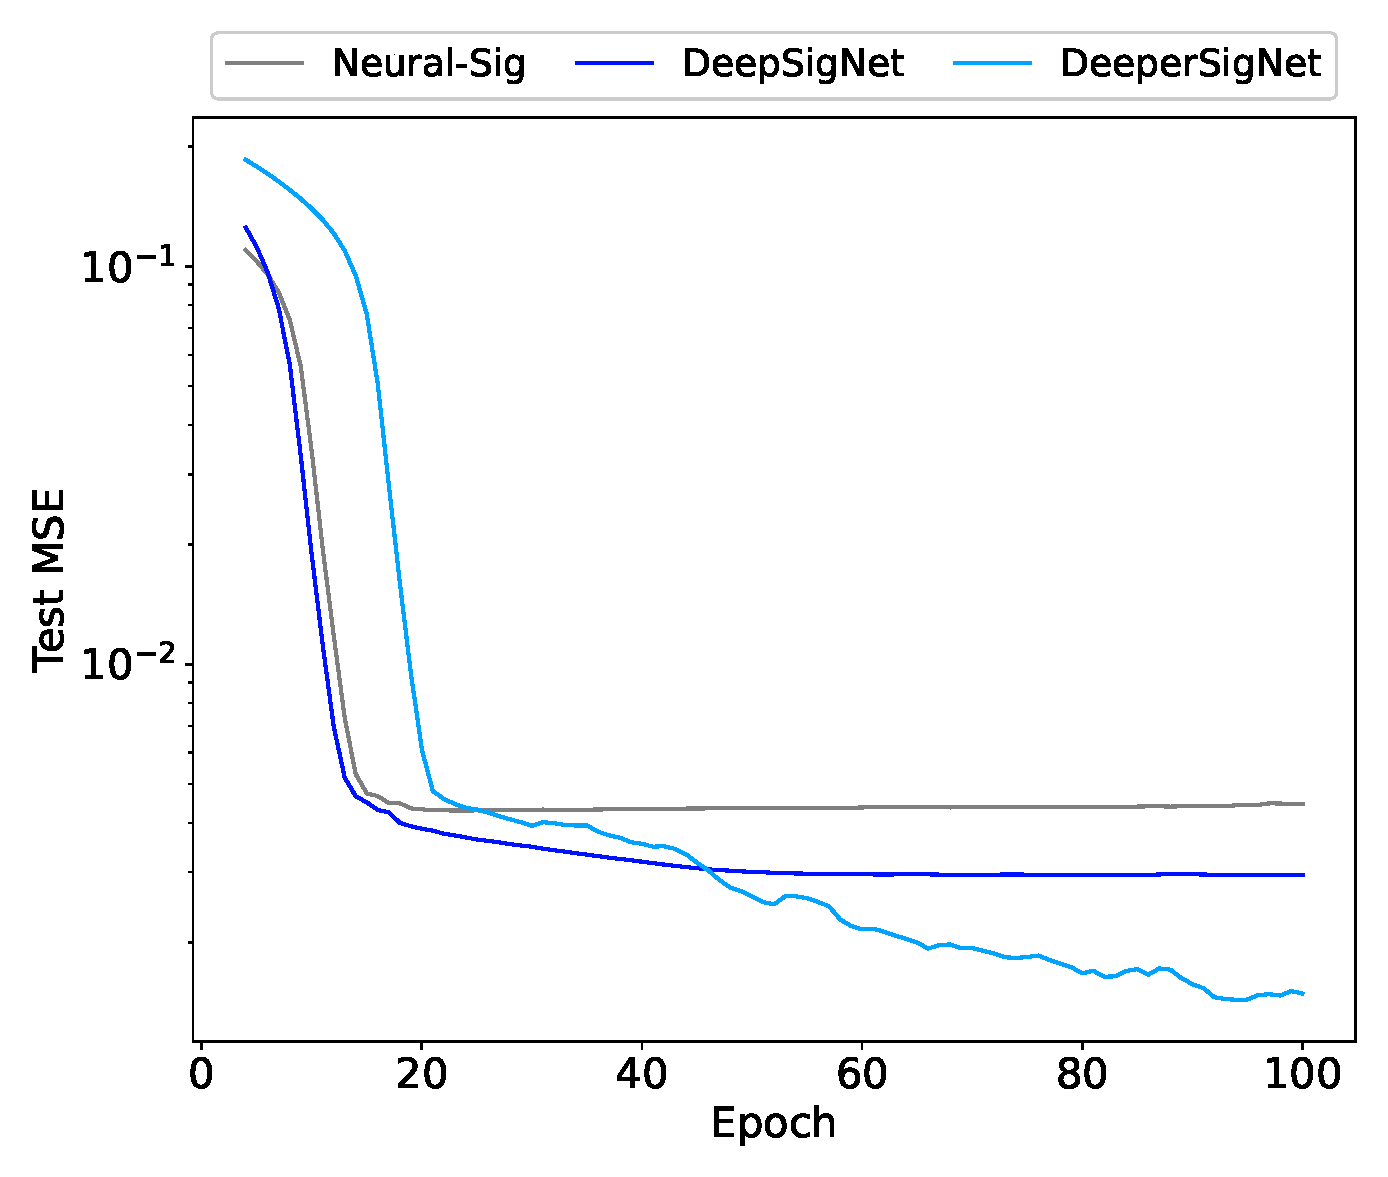
\includegraphics[width=0.32\textwidth]{fig//reproduce//difforder1.eps}}
	\subfigure[$N=2$.]{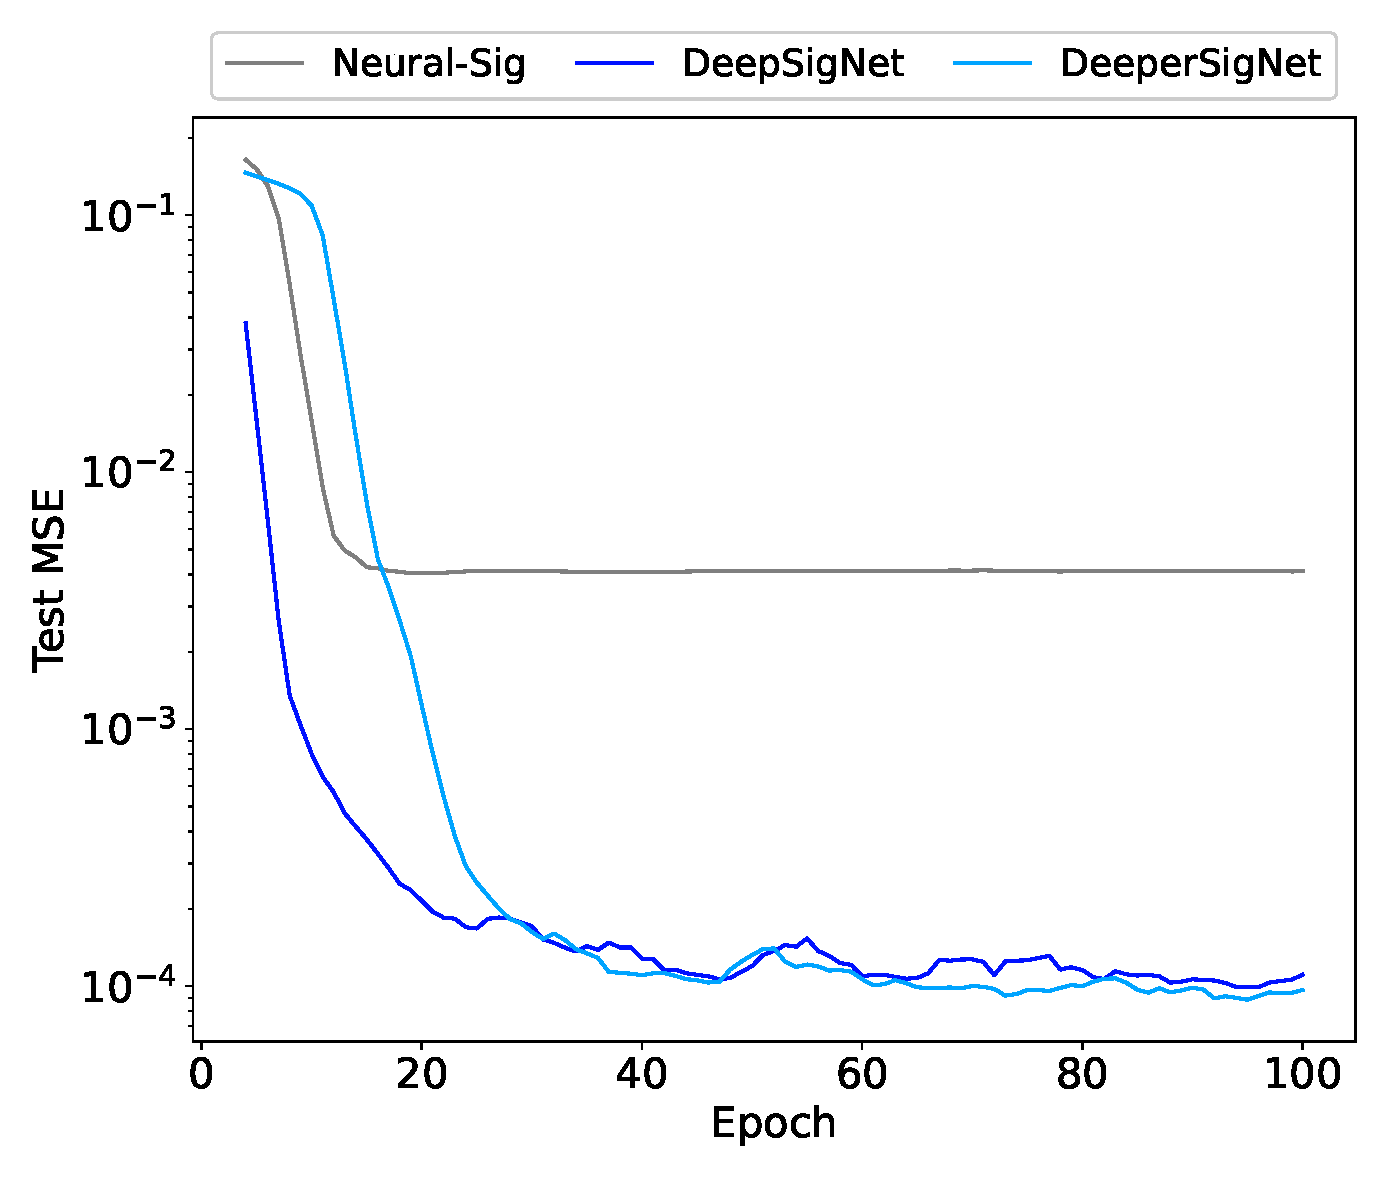
\includegraphics[width=0.32\textwidth]{fig//reproduce//difforder2.eps}}
	\subfigure[$N=3$.]{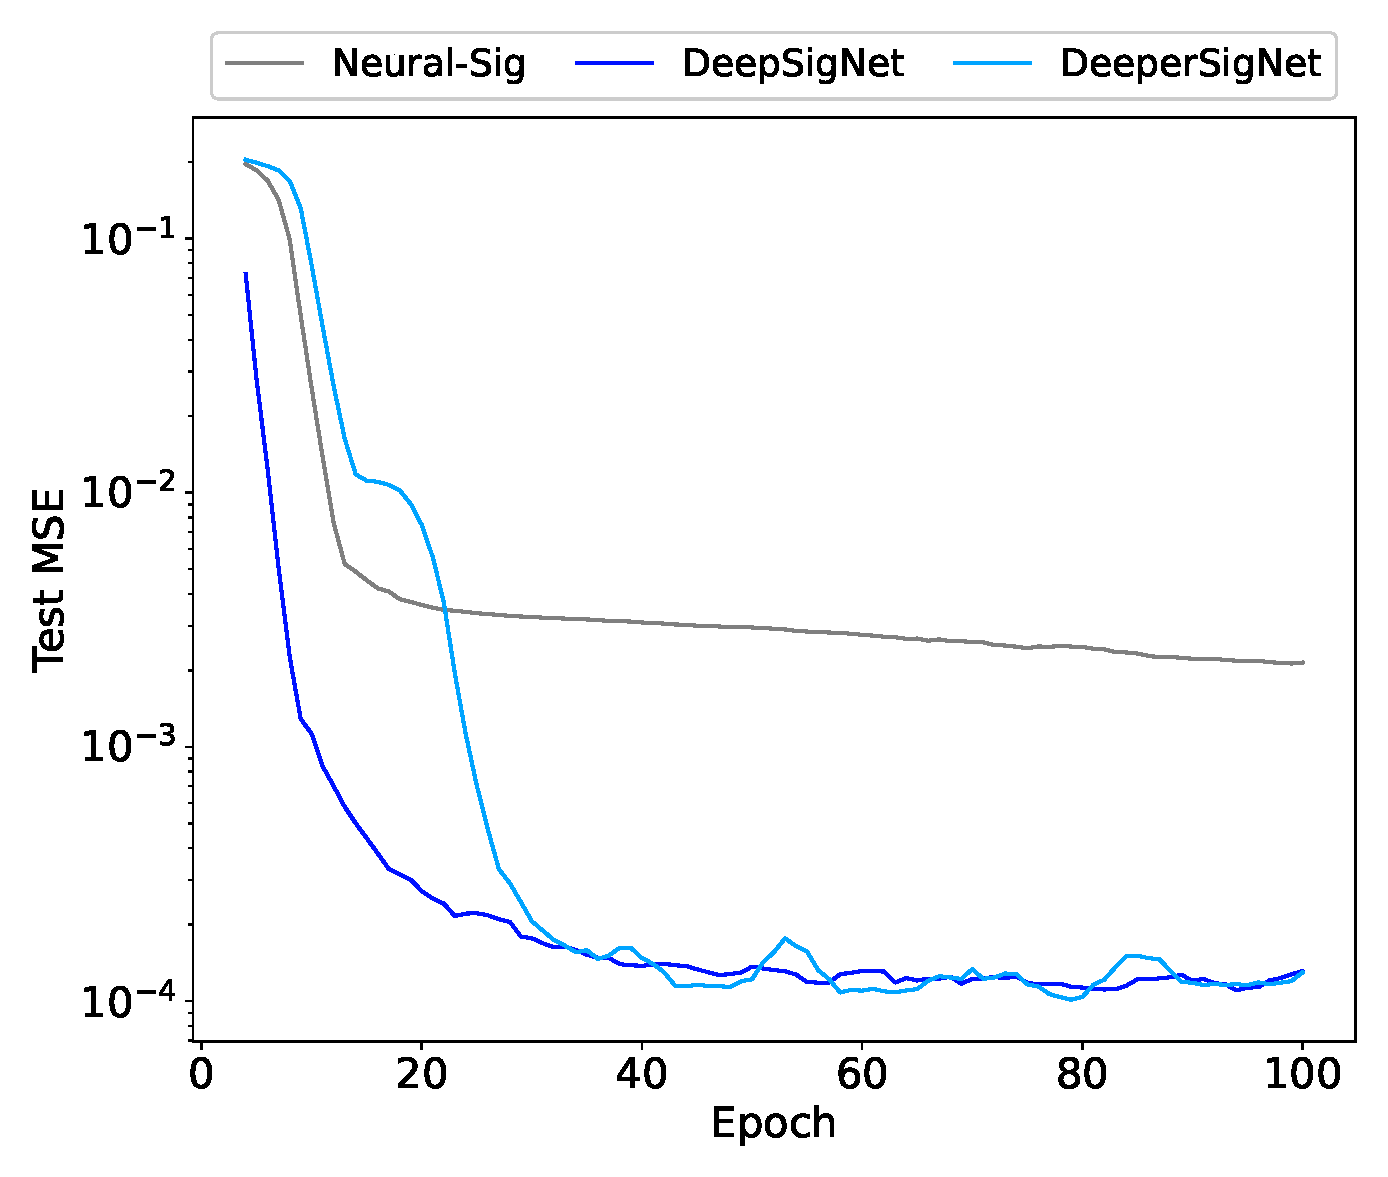
\includegraphics[width=0.32\textwidth]{fig//reproduce//difforder3.eps}}
	\subfigure[$N=4$.]{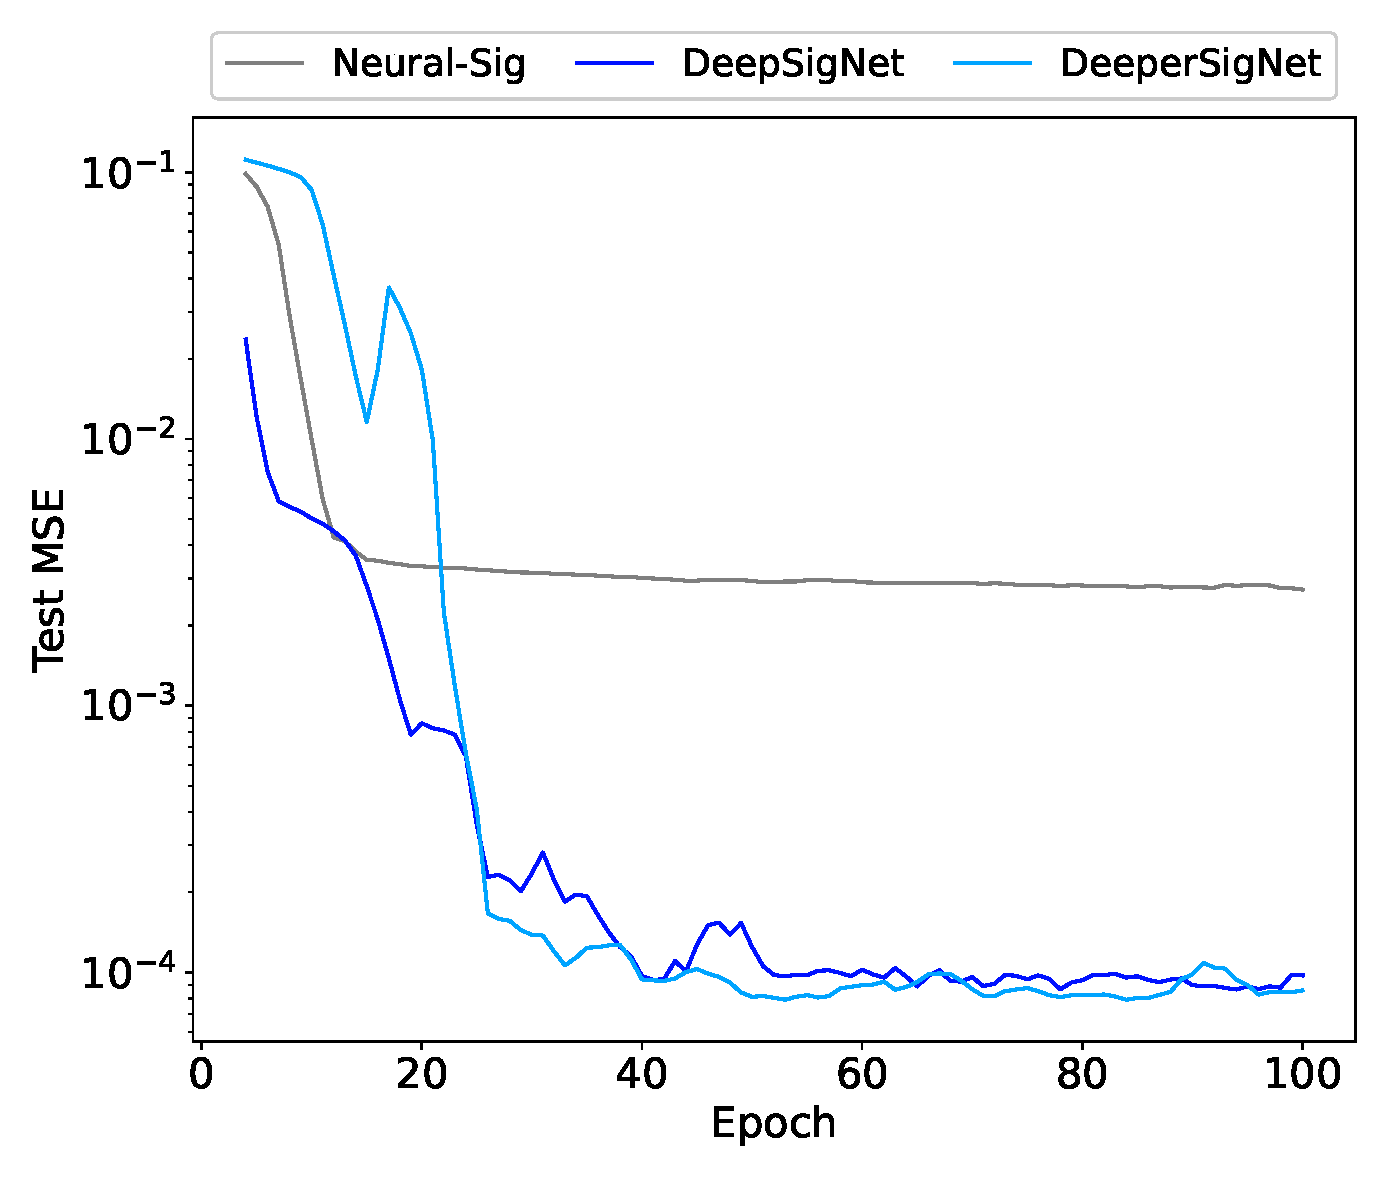
\includegraphics[width=0.32\textwidth]{fig//reproduce//difforder4.eps}}
	\subfigure[$N=5$.]{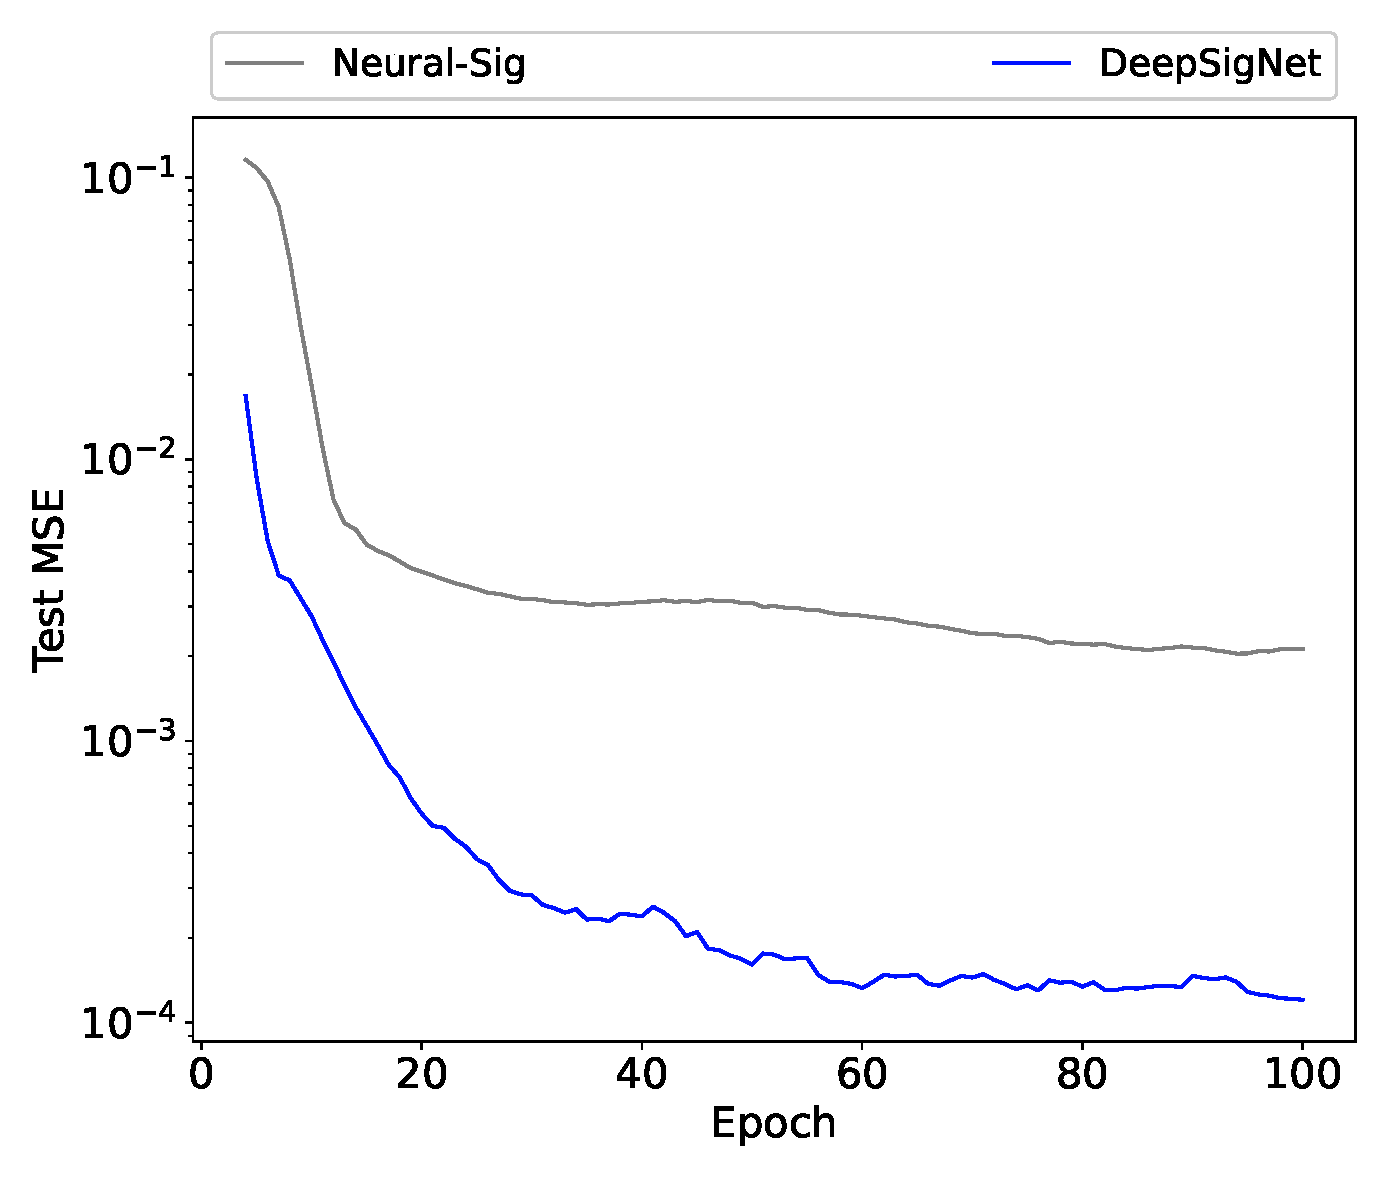
\includegraphics[width=0.32\textwidth]{fig//reproduce//difforder5.eps}}
	\subfigure[$N=6$.]{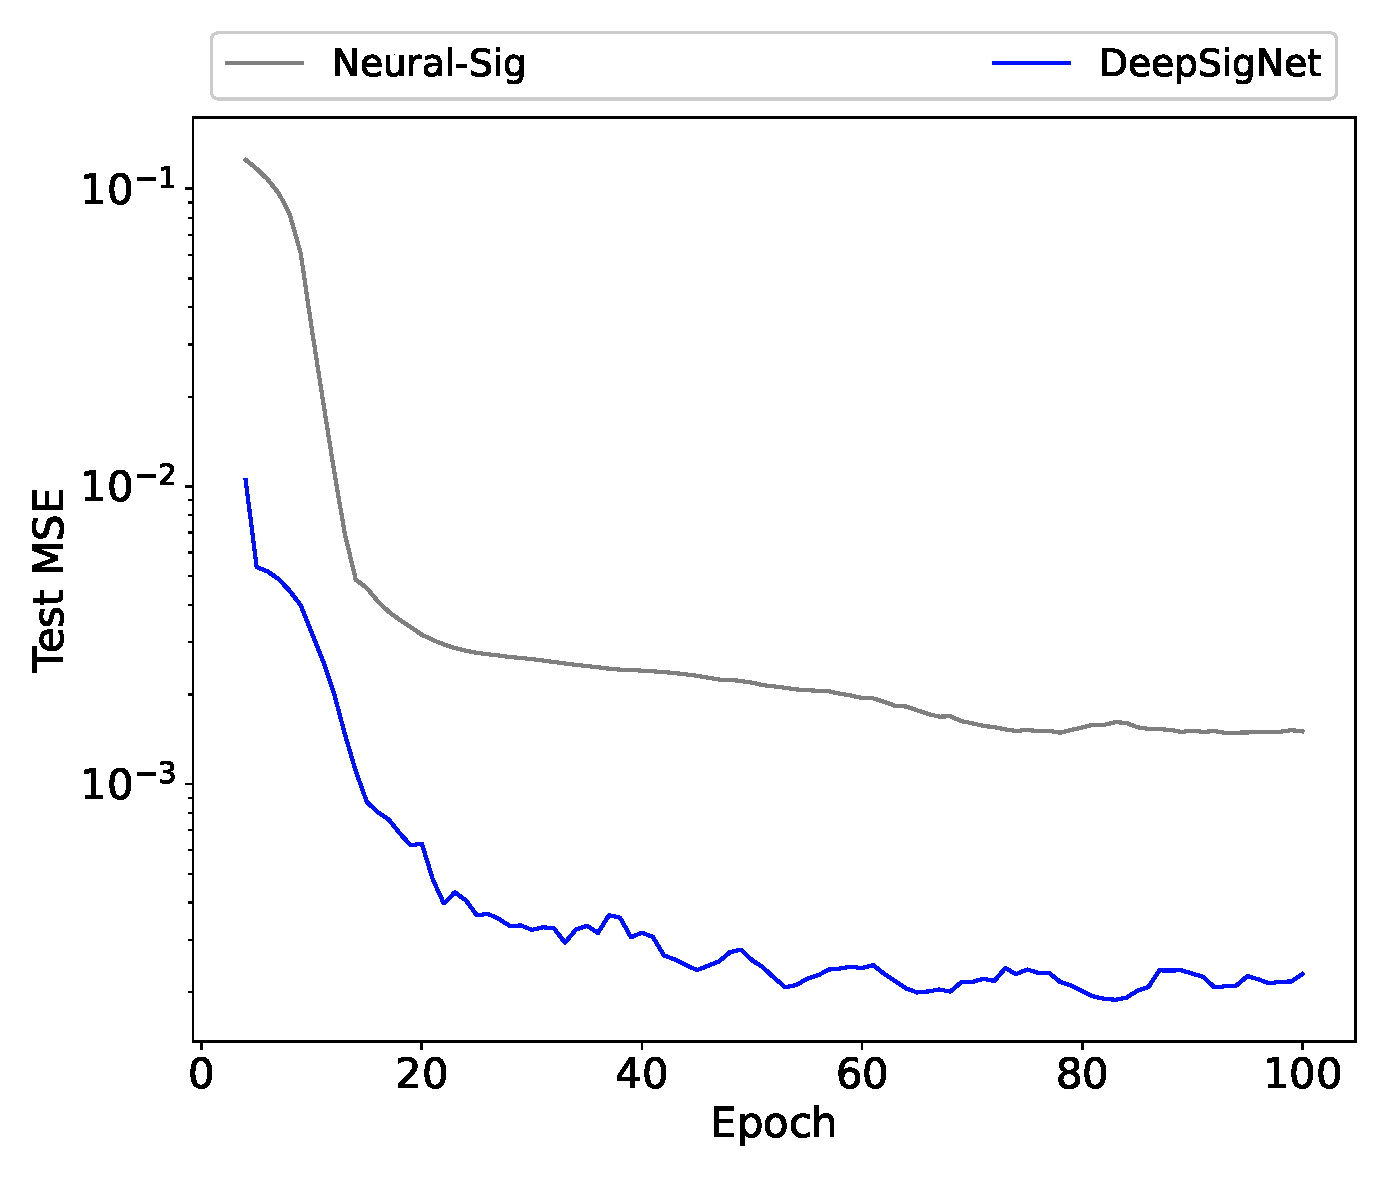
\includegraphics[width=0.32\textwidth]{fig//reproduce//difforder6.eps}}
	\caption{Performance at estimating the Hurst parameter with different signature truncation order $N$ for various models, with and without signatures, for a particular (typical) training run.}
	\label{fig-reproduce-difforder}
\end{figure}

\subsection{Supervised learning with rough Heston volatility model}
In this example, we use the rough Heston volatility model instead of the fractional Brownian motion to generate data sets. 
\begin{eqnarray*}
	V_t &=& V_0 + \frac{1}{\Gamma\(\frac{1}{2}+H\)}\int_0^t(t-s)^{H-\frac{1}{2}} \kappa_1 (\theta - V_s)\,ds \\
	&+& \frac{1}{\Gamma\(\frac{1}{2}+H\)}\int_0^t\(t-s\)^{H-\frac{1}{2}} \kappa_2 \epsilon\sqrt{V_s}\,dB_s,\quad t \in [0,T],
\end{eqnarray*}
where $\kappa_1,\, \kappa_2,\,\theta,\,\epsilon,\,V_0,\,T$ are all constants and $B_t$ is standard Brownian motion. In order to simulate this volatility process, we apply the fast algorithm proposed by \cite{ma_2022_fast} with uniform mesh $0=t_0< \cdots <t_n=T$, where $N$ is a positive integer. For comparison, we also introduce another simulation scheme proposed by (Markovian approximation) \cite{Bayer_2023_simulation}. Then we train a variety of models to learn the map from these realization data streams of volatility $V$ to Hurst parameter, i.e. $$((t_0, V_{t_0}),\ldots,(t_n, V_{t_n})) \mapsto H.$$

\subsubsection{Gaussian Volterra processes}

We first set $\kappa_1=0$ and remove $\sqrt{V}$ in the Ito integral i.e. the rough Heston volatility process become the Gaussian Volterra process. The other parameters are set as $\kappa_2 = 0.3,\,\epsilon = 0.3$ and $V_0=0$. All other settings are the same as illustration in \ref{sec1}. The results are shown as Table~\ref{tab-volatility-Gaussion} and Figure~\ref{fig-volatility-Gaussion}.

\begin{table}[H]
	\caption{Final test mean squared error (MSE) for different models, averaged over 3 training runs. }
	\label{tab-volatility-Gaussion}
	\smallskip
	\centering
	\renewcommand\arraystretch{1.5}
	\resizebox{0.9\textwidth}{!}{\begin{tabular}{l c c c c c c c}
			\toprule
			&\multicolumn{3}{c}{Fast Algorithm}& \multicolumn{3}{c}{Markovian Approximation}& \\
			\cline{2-7}
			&\multicolumn{2}{c}{Test MSE}& &\multicolumn{2}{c}{Test MSE}& & \\
			\cline{2-3}
			\cline{5-6}
			& Mean & Variance & CPU time & Mean & Variance & CPU time & $\#$Params \\
			\cline{2-8}
			Feedforward &$3.82 \times 10^{-3}$&$1.26 \times 10^{-7}$&2.97s&$3.77 \times 10^{-3}$&$8.09 \times 10^{-9}$&2.03s&10209\\	
			RNN &$3.77 \times 10^{-3}$&$1.32 \times 10^{-7}$&137.91s&$3.77 \times 10^{-3}$&$7.53 \times 10^{-8}$&129.49s&10091\\			
			DeepSigNet &$3.80 \times 10^{-4}$&$3.51 \times 10^{-9}$&56.42s&$5.45 \times 10^{-4}$&$1.64 \times 10^{-8}$&48.38s&9261\\			
			DeeperSigNet &$4.17 \times 10^{-4}$&$2.41 \times 10^{-8}$&1504.62s&$6.76 \times 10^{-4}$&$2.51 \times 10^{-8}$&1502.50s&9686\\
			LSTM &$3.76 \times 10^{-3}$&$1.25 \times 10^{-7}$&399.85s&$3.78 \times 10^{-3}$&$7.06 \times 10^{-8}$&182.08s&12961\\
			GRU &$3.76 \times 10^{-3}$&$1.03 \times 10^{-7}$&275.33s&$3.80 \times 10^{-3}$&$6.23 \times 10^{-8}$&261.49s&9729\\
			Neural-Sig &$3.74 \times 10^{-3}$&$1.13 \times 10^{-7}$&2.30s&$3.57 \times 10^{-3}$&$6.47 \times 10^{-9}$&2.24s&10097\\		
			\bottomrule
	\end{tabular}}
\end{table}

\begin{figure}[H]
	\centering
	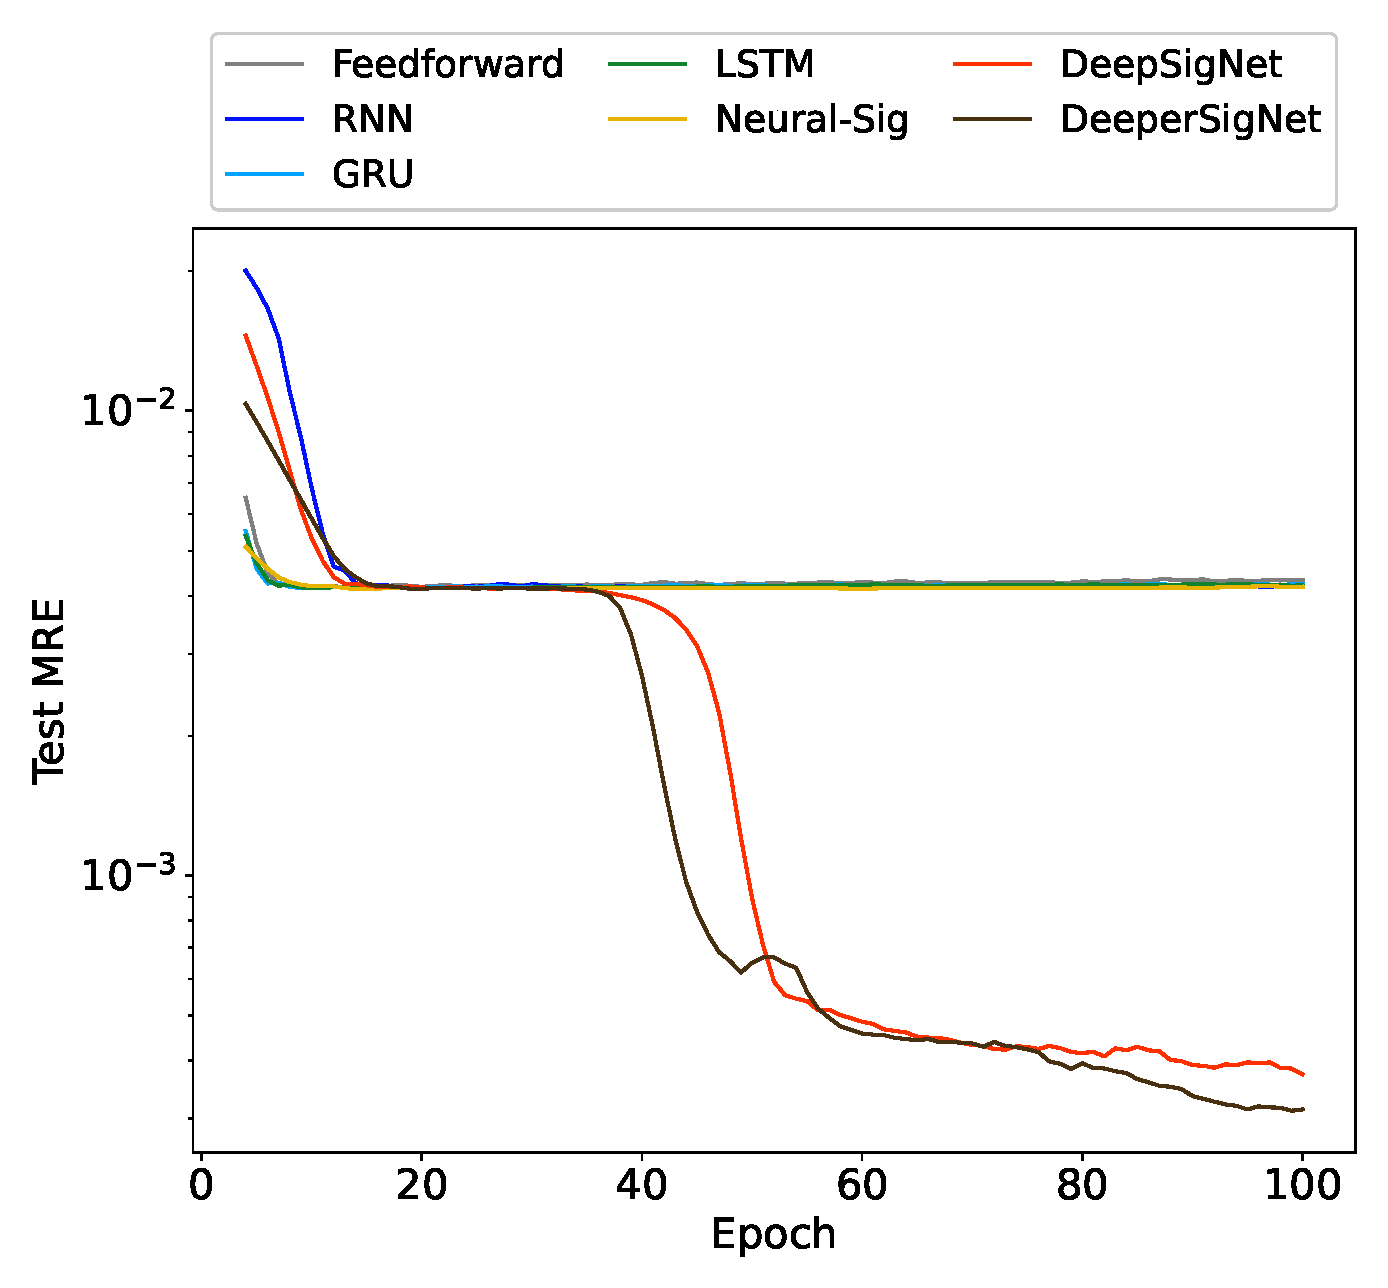
\includegraphics[width=0.49\textwidth]{fig//volatility//fast_Gaussion.eps}
	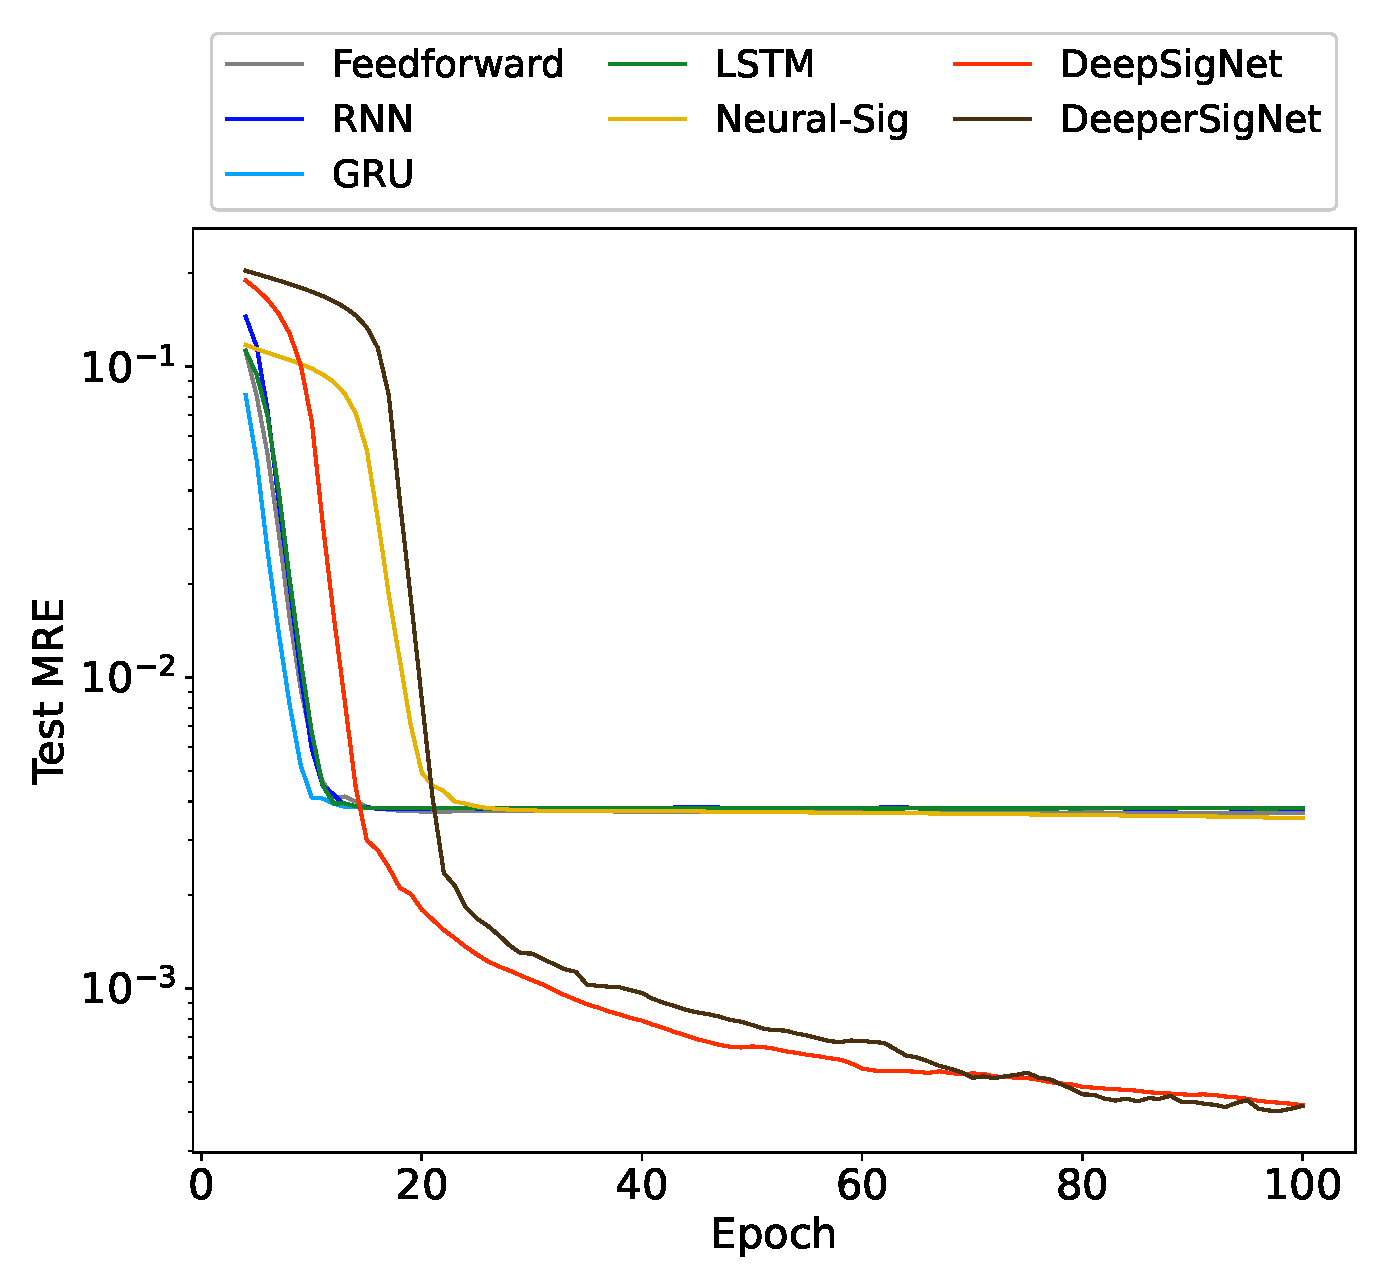
\includegraphics[width=0.49\textwidth]{fig//volatility//MarkovSimulation_Gaussion.eps}
	\caption{Performance at estimating the Hurst parameter for various models, with and without signatures, for a particular (typical) training run. Here, Fast Algorithm (left); Markovian Approximation (right). }
	\label{fig-volatility-Gaussion}
\end{figure}

The results appear to differ from those in \ref{original exp}. To explain this, we propose the paths of fractional Brownian motion and Gaussian Volterra process generated using different methods, as illustrated in Figure~\ref{fig-volatility-paths}. In contrast to fractional Brownian motion, when generating the rough Heston volatility process, non-negativity of values is required. If we allow the values of the Gaussian Volterra process to be negative and keep the same amplitude, the results would be consistent with those in \ref{original exp}.
\begin{figure}[H]
	\centering
	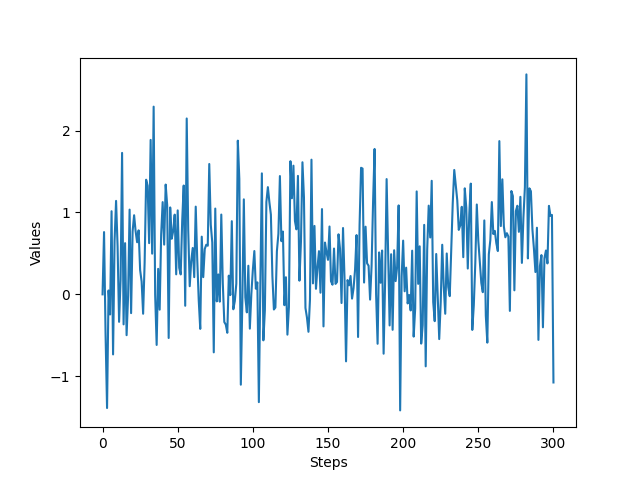
\includegraphics[width=0.32\textwidth]{fig//volatility//path_fbm.png}
	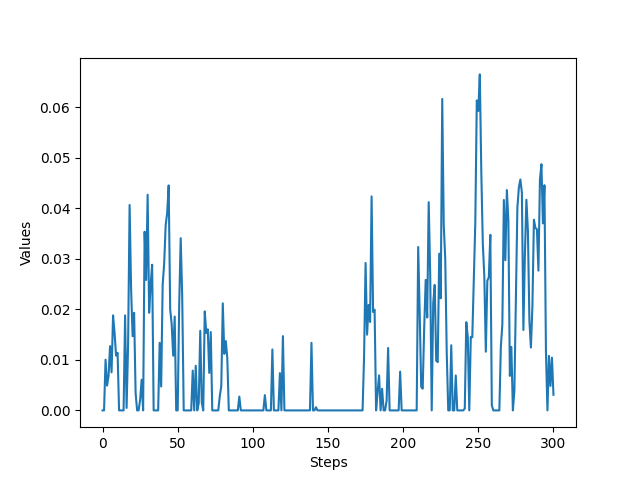
\includegraphics[width=0.32\textwidth]{fig//volatility//path_fast.png}
	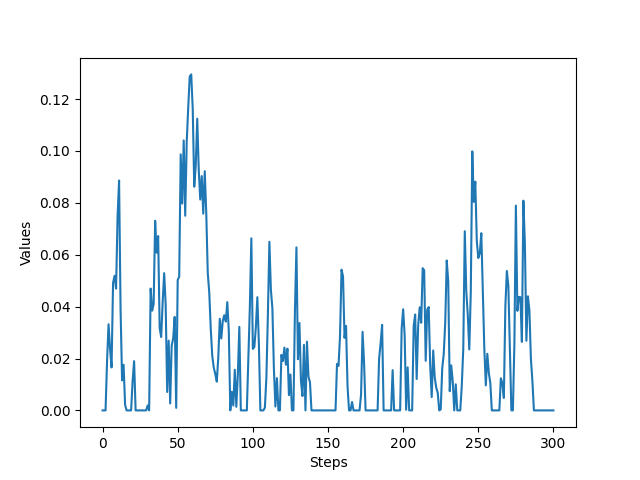
\includegraphics[width=0.32\textwidth]{fig//volatility//path_MarkovianApproximation.png}
	\caption{Paths of fractional Brownian motion and Gaussion Volterra process generated by Davies-Harte method (left), Fast Algorithm (middle) and Markovian Approximation (right). }
	\label{fig-volatility-paths}
\end{figure}

Next, we modify the Gaussian Volterra process by adding the $\sqrt{V}$ in the Ito integral and rerun this experiment. The results are shown as Table~\ref{tab-volatility-GaussionsqrtV} and Figure~\ref{fig-volatility-GaussionsqrtV}.
\begin{table}[H]
	\caption{Final test mean squared error (MSE) for different models, averaged over 3 training runs. }
	\label{tab-volatility-GaussionsqrtV}
	\smallskip
	\centering
	\renewcommand\arraystretch{1.5}
	\resizebox{0.9\textwidth}{!}{\begin{tabular}{l c c c c c c c}
					\toprule
					&\multicolumn{3}{c}{Fast Algorithm}& \multicolumn{3}{c}{Markovian Approximation}& \\
					\cline{2-7}
					&\multicolumn{2}{c}{Test MSE}& &\multicolumn{2}{c}{Test MSE}& & \\
					\cline{2-3}
					\cline{5-6}
					& Mean & Variance & CPU time & Mean & Variance & CPU time & $\#$Params \\
					\cline{2-8}
					Feedforward &$4.05 \times 10^{-3}$&$4.92 \times 10^{-8}$&4.61s&$4.11 \times 10^{-3}$&$3.49 \times 10^{-9}$&1.91s&10209\\	
					RNN &$4.03 \times 10^{-3}$&$5.06 \times 10^{-8}$&285.59s&$4.14 \times 10^{-3}$&$2.16 \times 10^{-9}$&136.08s&10091\\			
					DeepSigNet &$2.67 \times 10^{-4}$&$2.27 \times 10^{-9}$&62.68s&$1.85 \times 10^{-4}$&$3.73 \times 10^{-10}$&48.49s&9261\\			
					DeeperSigNet &$2.40 \times 10^{-4}$&$8.88 \times 10^{-10}$&2084.20s&$2.18 \times 10^{-4}$&$9.57 \times 10^{-9}$&1499.33s&9686\\
					LSTM &$3.99 \times 10^{-3}$&$9.56 \times 10^{-8}$&383.10s&$4.08 \times 10^{-3}$&$1.67 \times 10^{-9}$&193.08s&12961\\
					GRU &$4.01 \times 10^{-3}$&$7.89 \times 10^{-8}$&305.61s&$4.08 \times 10^{-3}$&$1.67 \times 10^{-9}$&245.32s&9729\\
					Neural-Sig &$4.00 \times 10^{-3}$&$7.93 \times 10^{-8}$&2.36s&$4.06 \times 10^{-3}$&$3.89 \times 10^{-9}$&2.36s&10097\\		
					\bottomrule
			\end{tabular}}
\end{table}

\begin{figure}[H]
	\centering
	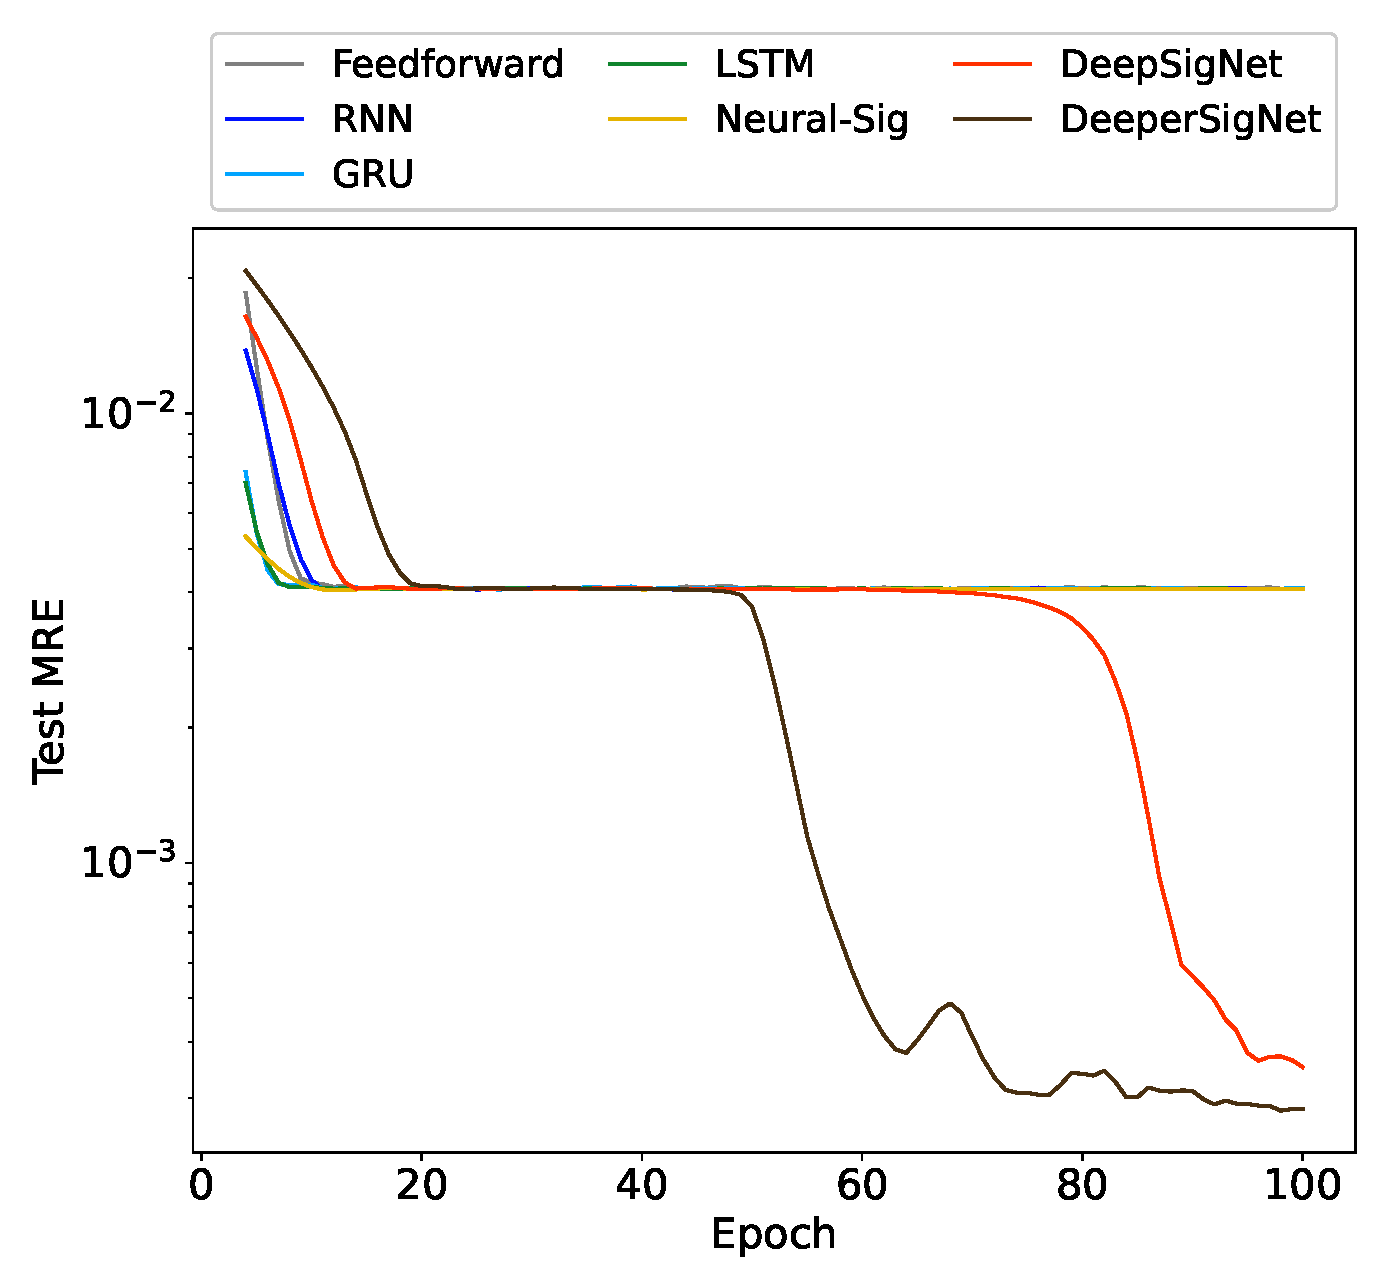
\includegraphics[width=0.49\textwidth]{fig//volatility//fast_GaussionsqrtV.eps}
	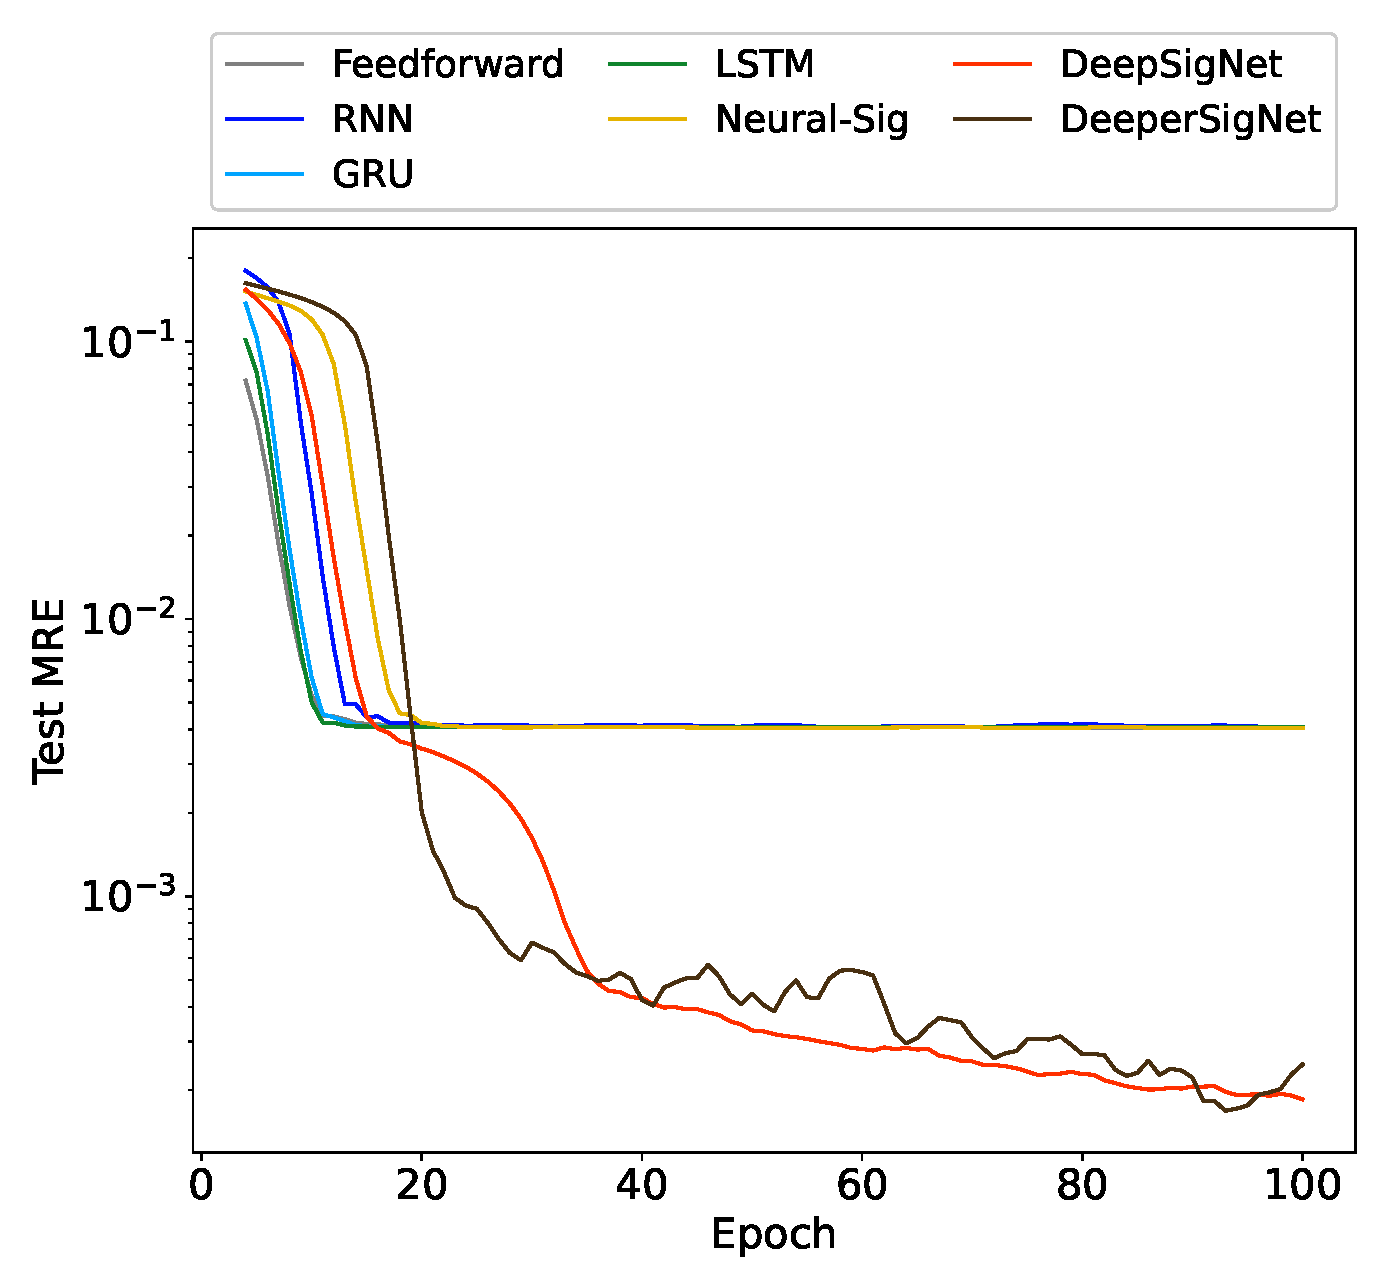
\includegraphics[width=0.49\textwidth]{fig//volatility//MarkovSimulation_GaussionsqrtV.eps}
	\caption{Performance at estimating the Hurst parameter for various models, with and without signatures, for a particular (typical) training run. Here, Fast Algorithm (left); Markovian Approximation (right). }
	\label{fig-volatility-GaussionsqrtV}
\end{figure}

\subsubsection{Single parameter calibration for rough Heston volatility processes}
Now, we consider the rough Heston volatility process. The parameters are set as $\kappa_1=\kappa_2 = 0.3,\,\theta=0.3,\,\epsilon = 0.3$ and $V_0=0$. The results are shown as Table~\ref{tab-volatility-V} and Figure~\ref{fig-volatility-V}.

\begin{table}[H]
	\caption{Final test mean squared error (MSE) for different models, averaged over 3 training runs. }
	\label{tab-volatility-V}
	\smallskip
	\centering
	\renewcommand\arraystretch{1.5}
	\resizebox{0.9\textwidth}{!}{\begin{tabular}{l c c c c c c c}
					\toprule
					&\multicolumn{3}{c}{Fast Algorithm}& \multicolumn{3}{c}{Markovian Approximation}& \\
					\cline{2-7}
					&\multicolumn{2}{c}{Test MSE}& &\multicolumn{2}{c}{Test MSE}& & \\
					\cline{2-3}
					\cline{5-6}
					& Mean & Variance & CPU time & Mean & Variance & CPU time & $\#$Params \\
					\cline{2-8}
					Feedforward &$3.96 \times 10^{-3}$&$4.88 \times 10^{-8}$&3.66s&$3.74 \times 10^{-3}$&$4.29 \times 10^{-9}$&1.95s&10209\\	
					RNN &$3.96 \times 10^{-3}$&$2.90 \times 10^{-8}$&265.48s&$4.25 \times 10^{-3}$&$1.77 \times 10^{-7}$&140.18s&10091\\			
					DeepSigNet &$2.86 \times 10^{-4}$&$1.22 \times 10^{-8}$&94.18s&$1.46 \times 10^{-4}$&$4.54 \times 10^{-10}$&84.93s&9261\\			
					DeeperSigNet &$2.50 \times 10^{-4}$&$1.86 \times 10^{-9}$&1767.80s&$1.83 \times 10^{-4}$&$7.02 \times 10^{-9}$&1533.53s&9686\\
					LSTM &$3.96 \times 10^{-3}$&$3.88 \times 10^{-8}$&435.44s&$4.23 \times 10^{-3}$&$1.68 \times 10^{-7}$&175.07s&12961\\
					GRU &$3.97 \times 10^{-3}$&$3.86 \times 10^{-8}$&320.01s&$4.21 \times 10^{-3}$&$1.60 \times 10^{-7}$&243.48s&9729\\
					Neural-Sig &$3.96 \times 10^{-3}$&$3.88 \times 10^{-8}$&2.38s&$3.97 \times 10^{-3}$&$1.08 \times 10^{-7}$&2.39s&10097\\		
					\bottomrule
			\end{tabular}}
\end{table}

\begin{figure}[H]
	\centering
	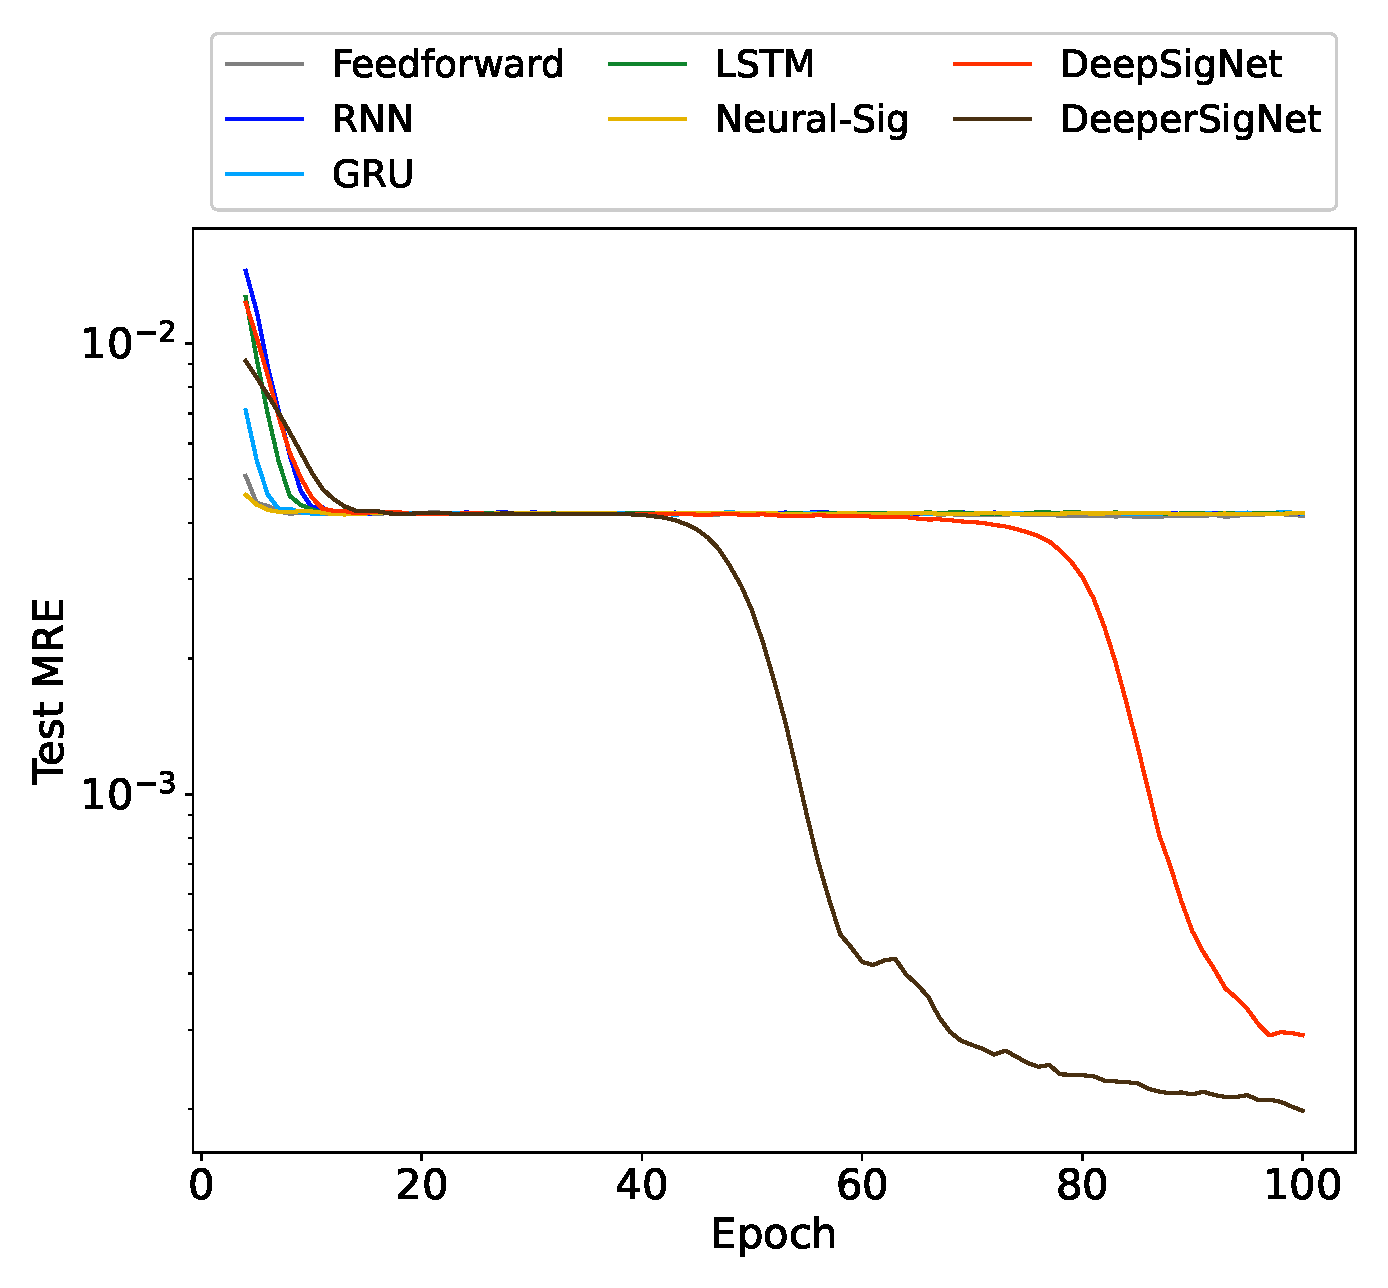
\includegraphics[width=0.49\textwidth]{fig//volatility//fast_V.eps}
	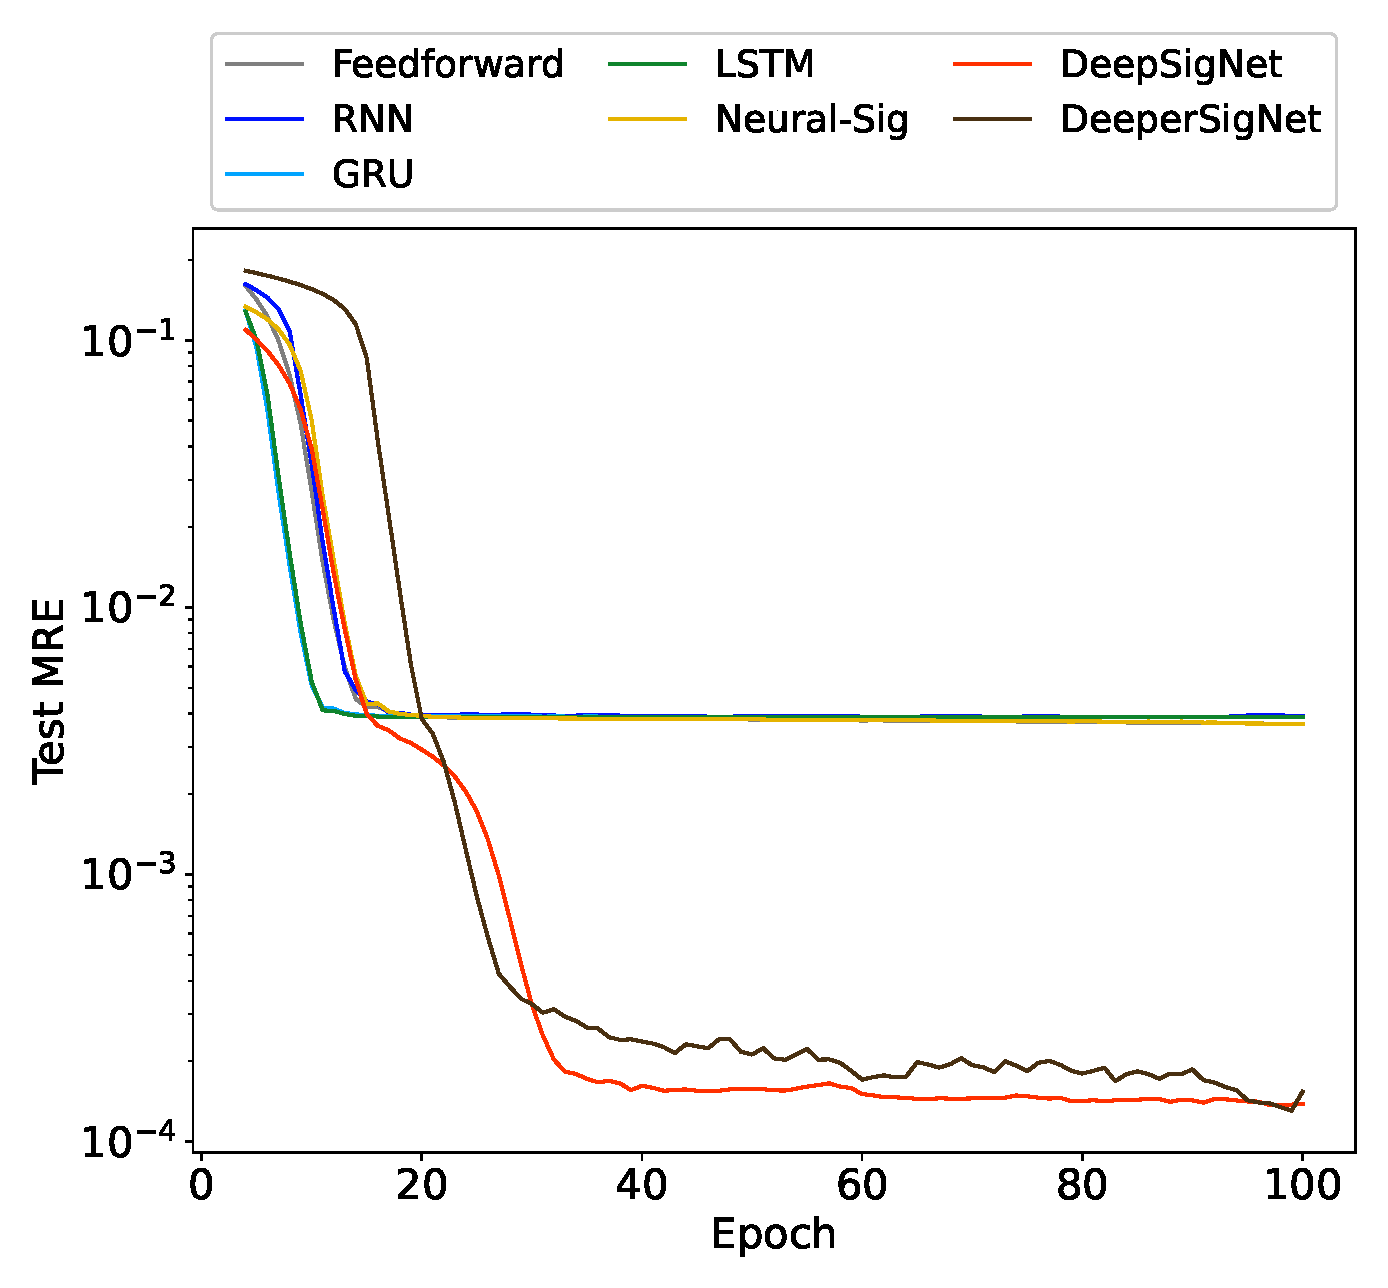
\includegraphics[width=0.49\textwidth]{fig//volatility//MarkovSimulation_V.eps}
	\caption{Performance at estimating the Hurst parameter for various models, with and without signatures, for a particular (typical) training run. Here, Fast Algorithm (left); Markovian Approximation (right). }
	\label{fig-volatility-V}
\end{figure}

Furthermore, we try to calibrate other parameters in rough Heston volatility processes such as $\kappa_2$. We use the fast algorithm to generate data set with $\kappa_2\in[0.1, 0.5],\,\kappa_1 = 0.3,\,\theta=0.3,\,\epsilon = 0.3,\, H=0.01$ and $V_0=0$. The results in Table~\ref{tab-rHeston-kappa} and Figure~\ref{fig-rHeston-kappa} clearly show that the DeepSigNet and DeeperSigNet outperform the other models, similar to the results in calibrating the Hurst parameter. 

\begin{table}[H]
	\caption{Final test mean squared error (MSE) for different models, averaged over 3 training runs, ordered from largest to smallest.}
	\label{tab-rHeston-kappa}
	\smallskip
	\centering
	\renewcommand\arraystretch{1.5}
	\resizebox{0.9\textwidth}{!}{\begin{tabular}{l c c c c}
			\toprule
			&\multicolumn{2}{c}{Test MSE} & & \\
			\cline{2-3}
			& Mean & Variance & $\#$Params & CPU time \\
			\cline{2-5}
			RNN &$6.51 \times 10^{-3}$&$7.00 \times 10^{-7}$&10091&155.18s\\
			LSTM &$5.27 \times 10^{-3}$&$1.44 \times 10^{-7}$&12961&590.72s\\
			GRU &$4.61 \times 10^{-3}$&$1.06 \times 10^{-7}$&9729&366.06s\\
			Neural-Sig &$3.20 \times 10^{-3}$&$1.60 \times 10^{-7}$&10097&2.24s\\
			Feedforward &$3.03 \times 10^{-3}$&$1.77 \times 10^{-7}$&10209&1.88s\\
			DeeperSigNet &$4.95 \times 10^{-4}$&$7.95 \times 10^{-8}$&9686&2448.63s\\
			DeepSigNet &$3.10 \times 10^{-4}$&$1.70 \times 10^{-9}$&9261&139.76s\\				
			\bottomrule
	\end{tabular}}
\end{table}

\begin{figure}[H]
	\centering
	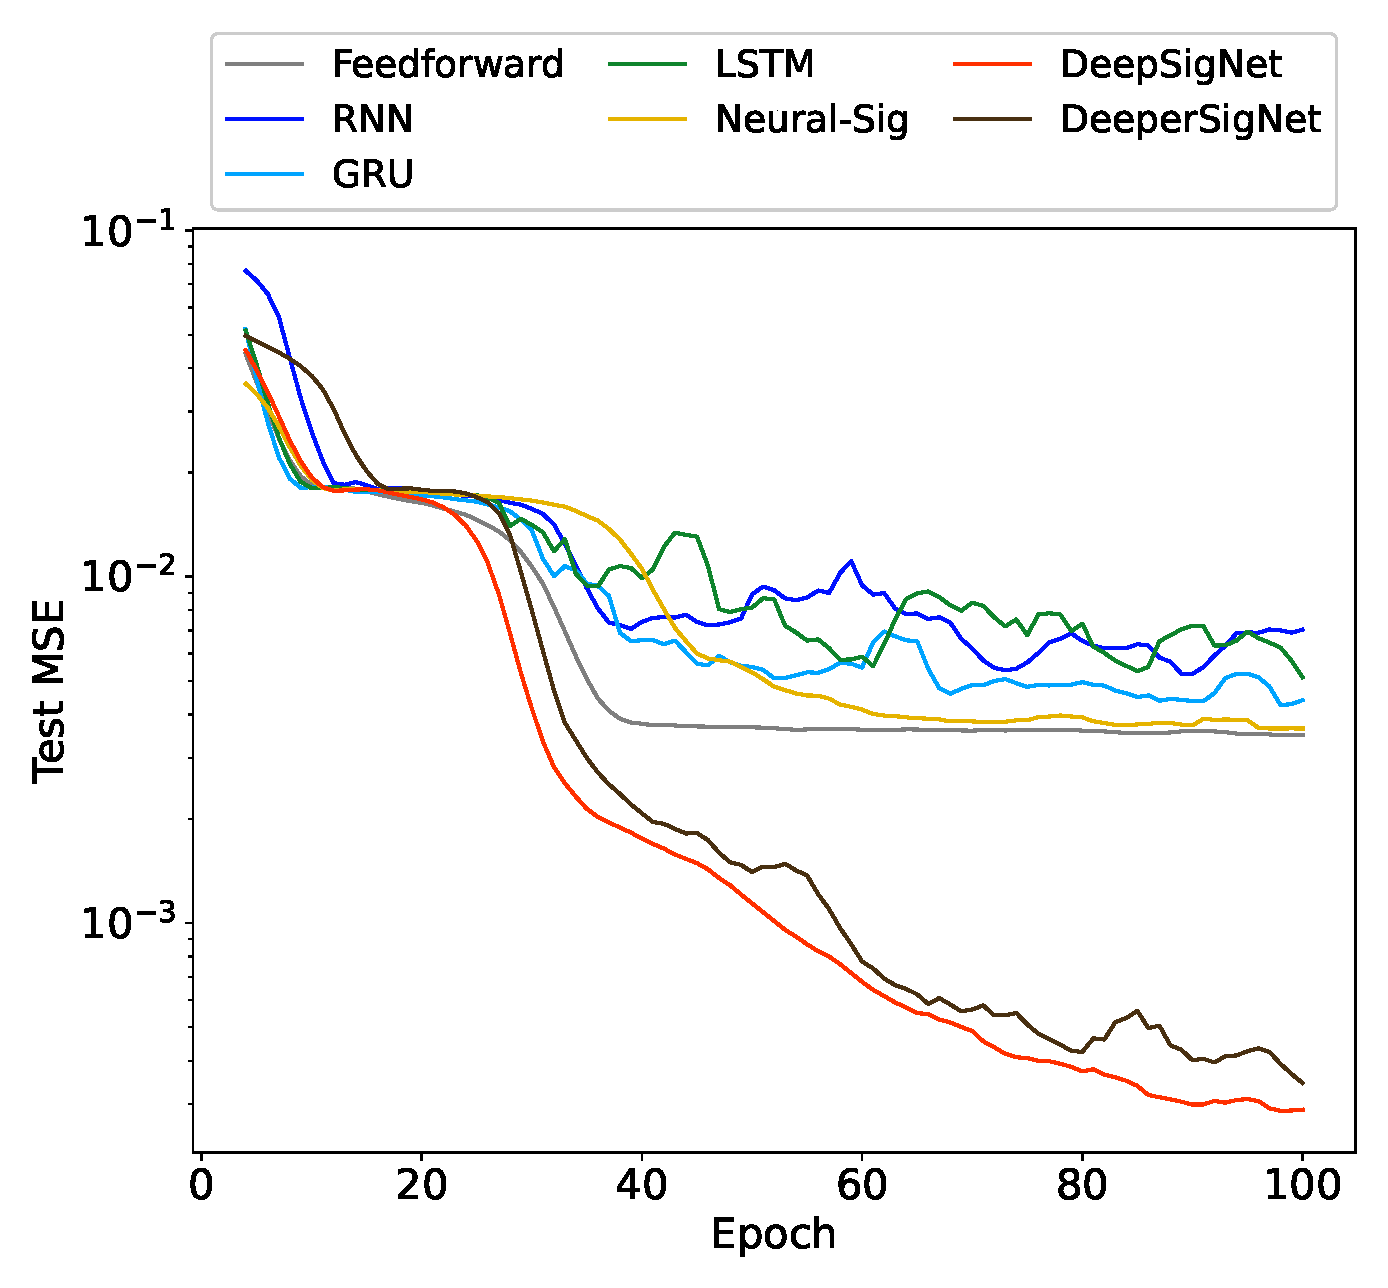
\includegraphics[width=0.8\textwidth]{fig//volatility//rHeston_V_kappa.eps}
	\caption{Performance at estimating the $\kappa_1$ for various models, with and without signatures, for a particular (typical) training run. }
	\label{fig-rHeston-kappa}
\end{figure}

\subsubsection{Multi-parameter calibration for rough Heston volatility processes}
In this example, we try to calibrate $\kappa_2$ and the Hurst parameter simultaneously. We use the fast algorithm to generate data set with $\kappa_2\in[0.1, 0.5],\,H\in\left(0,0.2\right],\,\kappa_1 = 0.3,\,\theta=0.3,\,\epsilon = 0.3$ and $V_0=0$. The results in Table~\ref{tab-rHeston-kappa&H} and Figure~\ref{fig-rHeston-kappa&H} show that the DeepSigNet and DeeperSigNet outperform the other models but the difference is not significant. We also attempted a higher signature truncation order, but there was no significant improvement.

\begin{table}[H]
	\caption{Final test mean squared error (MSE) for different models, averaged over 3 training runs, ordered from largest to smallest.}
	\label{tab-rHeston-kappa&H}
	\smallskip
	\centering
	\renewcommand\arraystretch{1.5}
	\resizebox{0.9\textwidth}{!}{\begin{tabular}{l c c c c}
			\toprule
			&\multicolumn{2}{c}{Test MSE} & & \\
			\cline{2-3}
			& Mean & Variance & $\#$Params & CPU time \\
			\cline{2-5}
			LSTM &$1.13 \times 10^{-2}$&$1.40 \times 10^{-6}$&12961&405.41s\\
			GRU &$1.01 \times 10^{-2}$&$7.18 \times 10^{-6}$&9729&471.15s\\
			RNN &$8.90 \times 10^{-3}$&$6.97 \times 10^{-6}$&10091&124.50s\\
			Neural-Sig &$8.58 \times 10^{-3}$&$8.66 \times 10^{-7}$&10097&2.24s\\
			Feedforward &$8.01 \times 10^{-3}$&$3.40 \times 10^{-7}$&10209&1.87s\\	
			DeepSigNet &$6.34 \times 10^{-3}$&$1.22 \times 10^{-7}$&9261&47.86s\\
			DeeperSigNet &$6.18 \times 10^{-3}$&$6.21 \times 10^{-8}$&9686&2121.87s\\					
			\bottomrule
	\end{tabular}}
\end{table}

\begin{figure}[H]
	\centering
	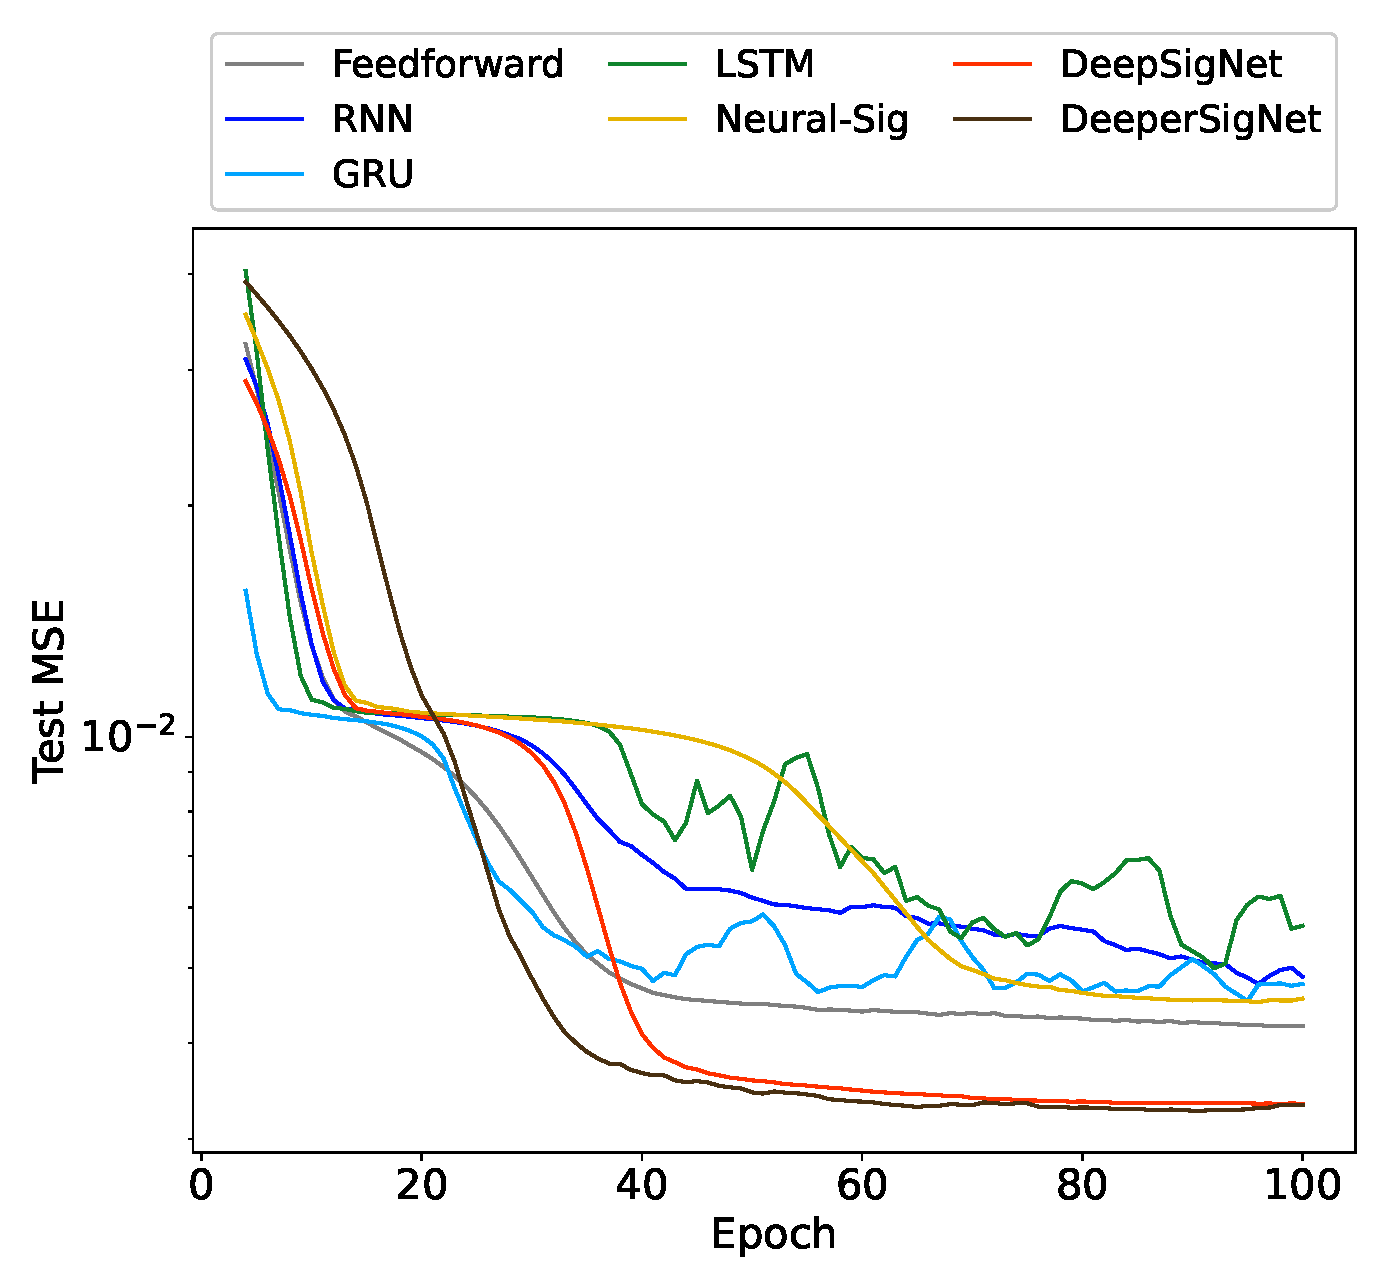
\includegraphics[width=0.8\textwidth]{fig//volatility//rHeston_V_kappaandH.eps}
	\caption{Performance at estimating the $\kappa_1$ and $H$ for various models, with and without signatures, for a particular (typical) training run. }
	\label{fig-rHeston-kappa&H}
\end{figure}

\subsection{Supervised learning with rough Bergomi volatility model}
In this example, we use the rough Bergomi (rBergomi) volatility process instead of rough Heston volatility process to generate data sets. The rBergomi volatility process is defined as
\begin{eqnarray*}
	V_t &=& V_0 \exp\left(\int_{0}^{t}\eta\sqrt{2H}(t-s)^{H-\frac{1}{2}}dW_s-\frac{\eta^2}{2} t^{2H}\right),\,V_0 > 0,
\end{eqnarray*}
where $W$ is a standard Brownian motion and $\eta$ is a strictly positive constant. Here we follow \cite{stone_2020} to use simulated sample paths of the normalized log volatility process ${(\log(V_t/V_0))}_{t\geq0}$ of the rBergomi model as the input data.

\subsubsection{Single parameter calibration for rough Bergomi volatility processes}
We first set $H\in\left(0,0.2\right]$ and $\eta = 1$ to generate data sets. The results in Table~\ref{tab-rBergomi-H} and Figure~\ref{fig-rBergomi-H} show that the DeepSigNet and DeeperSigNet outperform the other models. This result is similar to the result in \cite{stone_2020}, where a convolutional neural network was used with the root mean square error (RMSE) as the measure.

\begin{table}[H]
	\caption{Final test mean squared error (MSE) for different models, averaged over 3 training runs, ordered from largest to smallest.}
	\label{tab-rBergomi-H}
	\smallskip
	\centering
	\renewcommand\arraystretch{1.5}
	\resizebox{0.9\textwidth}{!}{\begin{tabular}{l c c c c}
			\toprule
			&\multicolumn{2}{c}{Test MSE} & & \\
			\cline{2-3}
			& Mean & Variance & $\#$Params & CPU time \\
			\cline{2-5}
			Feedforward &$2.67 \times 10^{-2}$&$1.06 \times 10^{-6}$&10209&3.47s\\
			LSTM &$2.25 \times 10^{-2}$&$1.37 \times 10^{-4}$&12961&246.62s\\
			Neural-Sig &$7.10 \times 10^{-3}$&$8.89 \times 10^{-7}$&10097&2.40s\\
			RNN &$3.67 \times 10^{-3}$&$7.87 \times 10^{-7}$&10091&108.44s\\
			GRU &$2.09 \times 10^{-3}$&$3.41 \times 10^{-7}$&9729&259.43s\\	
			DeepSigNet &$3.32 \times 10^{-4}$&$5.19 \times 10^{-8}$&9261&48.18s\\
			DeeperSigNet &$3.16 \times 10^{-4}$&$7.13 \times 10^{-9}$&9686&1669.37s\\			
			\bottomrule
	\end{tabular}}
\end{table}

\begin{figure}[H]
	\centering
	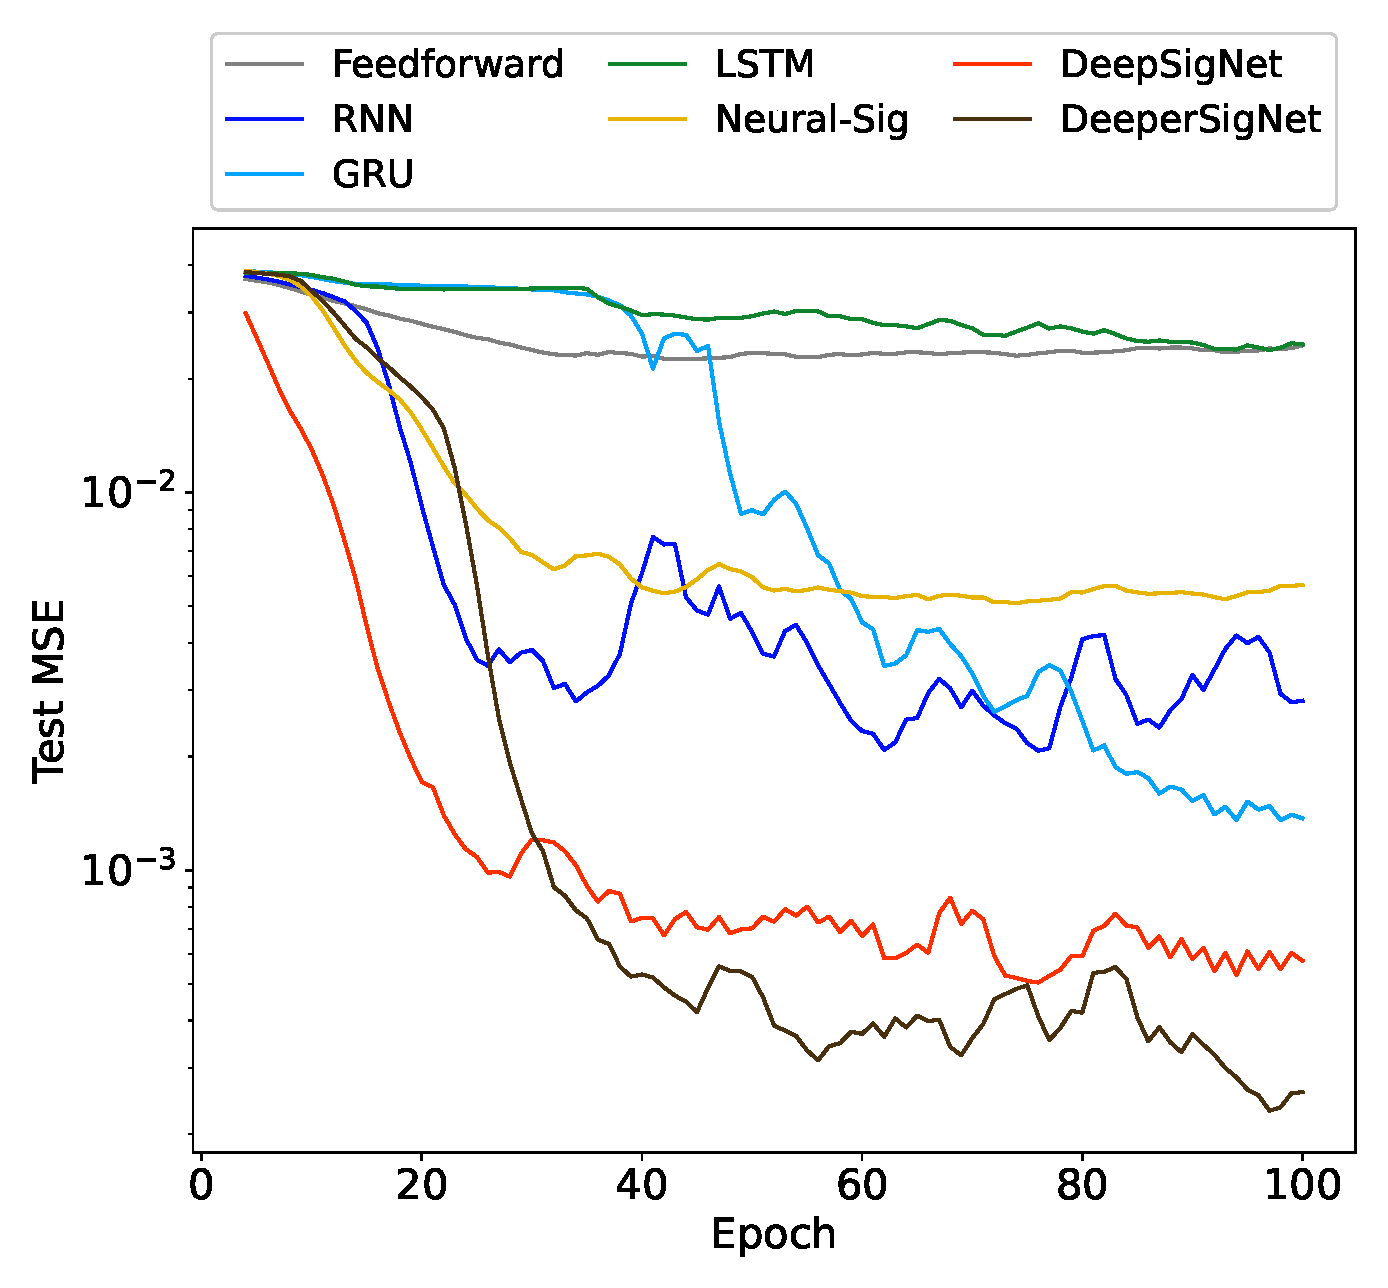
\includegraphics[width=0.8\textwidth]{fig//volatility//rBergomi_V_H.eps}
	\caption{Performance at estimating the Hurst parameter for various models, with and without signatures, for a particular (typical) training run. }
	\label{fig-rBergomi-H}
\end{figure}

%References
\begin{thebibliography}{10}
\bibitem[\protect\citeauthoryear{Bayer and Breneis}{2023}]{Bayer_2023_simulation}
Bayer, C., and Breneis, S. (2023). Efficient option pricing in the rough Heston model using weak simulation schemes. arXiv preprint arXiv:2310.04146.

\bibitem[\protect\citeauthoryear{Kidger, Bonnier, Perez Arribas, Salvi and Lyons}{2019}]{Lyons_2019_DeepSignature}
Kidger, P., Bonnier, P., Perez Arribas, I., Salvi, C., and Lyons, T. (2019). Deep signature transforms. Advances in Neural Information Processing Systems, 32.

\bibitem[\protect\citeauthoryear{Ma and Wu}{2022}]{ma_2022_fast}
Ma, J. and Wu, H. (2022). A fast algorithm for simulation of rough volatility models. Quantitative Finance, 22, 447--462.

\bibitem[\protect\citeauthoryear{Stone}{2020}]{stone_2020}
Stone, H. (2020). Calibrating rough volatility models: a convolutional neural network approach. Quantitative Finance, 20(3), 379-392.

\end{thebibliography}
\end{document}
